% Laporan Tugas Besar 2 IF3170 Inteligensi Artifisial
% Kompilasi: lihat docs/laporan/README.md (pdflatex dua kali, atau build.bat / build.sh)

\documentclass[11pt,a4paper,oneside]{report}

% ---------------------------------------------------------------- paket
\usepackage[utf8]{inputenc}
\usepackage[T1]{fontenc}
\usepackage{lmodern}
\usepackage[a4paper,margin=2.5cm]{geometry}
\usepackage{amsmath,amssymb}
\usepackage{graphicx}
\usepackage{booktabs}
\usepackage{tabularx}
\usepackage{longtable}
\usepackage{array}
\usepackage{multirow}
\usepackage{float}
\usepackage{caption}
\usepackage{enumitem}
\usepackage{xcolor}
\usepackage{listings}
\usepackage{textcomp}
\usepackage[hidelinks]{hyperref}

\graphicspath{{gambar/}}
% nama kode panjang boleh dipenggal setelah garis bawah
\let\garisbawahasli\_
\renewcommand{\_}{\garisbawahasli\allowbreak}
\setlength{\parskip}{0.4em}
\setlength{\parindent}{0pt}
\setlist{itemsep=0.15em, topsep=0.3em}
\renewcommand{\arraystretch}{1.15}

% ---------------------------------------------------------------- istilah bahasa Indonesia (tanpa babel)
\renewcommand{\chaptername}{Bab}
\renewcommand{\contentsname}{Daftar Isi}
\renewcommand{\listfigurename}{Daftar Gambar}
\renewcommand{\listtablename}{Daftar Tabel}
\renewcommand{\figurename}{Gambar}
\renewcommand{\tablename}{Tabel}
\renewcommand{\appendixname}{Lampiran}
\renewcommand{\bibname}{Referensi}
\renewcommand{\lstlistingname}{Kode}

% ---------------------------------------------------------------- kode program
\definecolor{kodeabu}{gray}{0.96}
\definecolor{kodekomentar}{rgb}{0.25,0.45,0.25}
\definecolor{kodekata}{rgb}{0.10,0.20,0.60}
\definecolor{kodestring}{rgb}{0.60,0.15,0.15}
\lstset{
  language=Python,
  basicstyle=\ttfamily\footnotesize,
  keywordstyle=\color{kodekata}\bfseries,
  commentstyle=\color{kodekomentar}\itshape,
  stringstyle=\color{kodestring},
  backgroundcolor=\color{kodeabu},
  numbers=left, numberstyle=\tiny\color{gray}, numbersep=6pt,
  frame=single, rulecolor=\color{gray!40},
  breaklines=true, breakatwhitespace=true,
  showstringspaces=false, upquote=true, columns=fullflexible,
  tabsize=4, xleftmargin=1.5em, framexleftmargin=1.5em,
}

% ---------------------------------------------------------------- penanda bagian yang belum diisi
\newcommand{\todo}[1]{\textcolor{red}{\textbf{[TODO: #1]}}}

\begin{document}

\ifdefined\NaiveBayesOnly
\renewcommand{\thesection}{\arabic{section}}
\renewcommand{\theequation}{\arabic{equation}}
\renewcommand{\thefigure}{\arabic{figure}}
\renewcommand{\thetable}{\arabic{table}}
\renewcommand{\thelstlisting}{\arabic{lstlisting}}
\begin{center}
  {\large IF3170 Inteligensi Artifisial \enspace|\enspace Tugas Besar 2\par}
  \vspace{0.6cm}
  {\LARGE\bfseries Categorical Naive Bayes\par}
  \vspace{0.2cm}
  {\large Prediksi Pembatalan Pemesanan Penginapan\par}
  \vspace{0.4cm}
  Arghawisesa Dwinanda Arham (13524100)\\
  Kelompok 17 -- DerbyCounty \enspace|\enspace Institut Teknologi Bandung
\end{center}
\vspace{0.3cm}

\section{Dasar Teori}
Categorical Naive Bayes memperkirakan peluang pembatalan dari kode kategori setiap fitur. Target \(Y\) bernilai 1 untuk pemesanan yang batal dan 0 untuk pemesanan yang tidak batal. Model mengasumsikan bahwa fitur \(X_1,\ldots,X_m\) saling independen setelah kelas diketahui \cite{ref:bayesnet}. Dengan asumsi tersebut, posterior sebanding dengan prior kelas dikalikan peluang setiap kategori pada kelas itu:
\begin{equation}
  P(Y=c\mid x) \propto P(Y=c)\prod_{j=1}^{m} P(X_j=x_j\mid Y=c).
\end{equation}
Prior \(P(Y=c)\) diestimasi dari proporsi kelas pada data latih. Peluang kategori diestimasi dengan \emph{additive smoothing} \cite{ref:categoricalnb}:
\begin{equation}
  P(X_j=v\mid Y=c)=\frac{N_{j,v,c}+\alpha_j}{N_c+\alpha_j K_j}.
\end{equation}
\(N_{j,v,c}\) adalah jumlah baris kelas \(c\) dengan kategori \(v\) pada fitur \(j\), \(N_c\) adalah jumlah baris kelas tersebut, dan \(K_j\) adalah jumlah kode kategori yang dicakup tabel fitur. Smoothing mencegah peluang nol untuk kategori yang tidak muncul pada kelas tertentu. Laplace smoothing adalah kasus \(\alpha_j=1\).

Untuk menghindari \emph{underflow}, perkalian diubah menjadi penjumlahan logaritma. Eksperimen berbobot memakai \(s_c=\log P(Y=c)+\sum_j w_j\log P(X_j=x_j\mid Y=c)\). Bobot \(w_j>1\) memperkuat kontribusi fitur tersebut terhadap perbandingan skor kelas \cite{ref:zaidi_nb}. Model menormalkan kedua skor setelah mengurangi nilai maksimum dan memprediksi kelas 1 ketika hasil normalisasi untuk kelas 1 mencapai threshold. Pada baseline dan model kontekstual, semua bobot bernilai 1.

\section{Implementasi}
Empat tahap eksperimen memakai notebook mandiri di \texttt{src/experiments/nb/} pada branch \texttt{main}. Setiap tahap mengimplementasikan \texttt{fit(X, y)}, \texttt{predict\_proba(X)}, dan \texttt{predict(X, threshold)} dengan NumPy. \texttt{fit} menyimpan log-prior kelas dan satu tabel log-likelihood untuk setiap kolom. \texttt{predict\_proba} mengambil nilai dari tabel sesuai kode kategori pada baris tersebut, lalu menormalkan skor kelas. Kode~\ref{lst:nb_count} menunjukkan inti perhitungan varian kontekstual.

\noindent\begin{minipage}{\textwidth}
\begin{lstlisting}[caption={Penghitungan log-likelihood dan skor Naive Bayes (cuplikan)},label={lst:nb_count}]
def categorical_counts(codes, y):
    n_categories = max(2, int(codes.max()) + 1)
    indices = y * n_categories + codes.astype(np.intp, copy=False)
    counts = np.bincount(indices, minlength=2 * n_categories)
    return counts.reshape(2, n_categories)

def categorical_log_likelihoods(counts, class_counts, alpha):
    alpha = np.asarray(alpha)[..., None, None]
    return np.log((counts + alpha) /
                  (class_counts[:, None] + alpha * counts.shape[1]))

# Di dalam predict_proba, setelah validasi masukan.
log_scores = np.empty((len(X), 2))
for label in (0, 1):
    log_scores[:, label] = self.log_prior_[label]
    for column, table in enumerate(self.log_likelihoods_):
        log_scores[:, label] += table[label, X[:, column]]
weights = np.exp(log_scores - log_scores.max(axis=1, keepdims=True))
return weights[:, 1] / weights.sum(axis=1)
\end{lstlisting}
\end{minipage}

\subsection{Baseline dan tuning dengan preprocessing tetap}
Dataset memuat 27.373 baris latih, 6.844 baris uji, dan 17 fitur pemesanan. \texttt{clean\_train} membuang 64 duplikat persis berdasarkan fitur dan target, tanpa menggunakan ID untuk mengidentifikasi duplikat. Preprocessor mengeluarkan kolom ID dan target dari masukan model dan mengubah \texttt{num\_adults = 0} menjadi nilai kosong. \texttt{NBPreprocessor} memakai \texttt{pd.cut} untuk membentuk tiga rentang \emph{lead time} (batas 30 dan 90 hari) serta tiga rentang tarif (batas Rp1 juta dan Rp2 juta). Nilai diskret lain langsung menjadi kategori. Kanal, tipe kamar, dan paket makan yang muncul kurang dari 20 kali pada data fit masuk \texttt{Other}. Kode 0 dicadangkan untuk kategori baru atau langka dan kode 1 untuk kategori kosong. Kamus dipelajari dari bagian latih setiap fold.

\begin{enumerate}
  \item \textbf{Baseline (\texttt{nb\_baseline}).} Seluruh 17 fitur dipakai, dengan \(\alpha=1\), bobot seragam, dan pilihan threshold dari prediksi OOF.
  \item \textbf{Fine-tuning (\texttt{nb\_baseline\_finetune}).} Preprocessing sama. Pencarian menguji 12 nilai alpha dan masing-masing enam bobot untuk \emph{lead time} dan jumlah permintaan khusus, sehingga ada 432 kombinasi sebelum pemilihan threshold. Bobot bekerja pada log-likelihood dan dipilih dengan Macro F1 OOF, mengikuti gagasan pembobotan atribut \cite{ref:zaidi_nb}. Konfigurasi terpilih memakai \(\alpha=2\), bobot 1 untuk \emph{lead time}, dan bobot 2 untuk \texttt{special\_requests}.
  \item \textbf{Smoothing per fitur (\texttt{nb\_baseline\_finetune\_2}).} Preprocessing, bobot, threshold 0,49, dan fold sama dengan tahap kedua. Hanya \(\alpha_{\text{permintaan}}\) yang diubah dari 2 ke 10. Uji ini mengukur dampak smoothing yang lebih kuat pada tabel kategori fitur yang mendapat bobot 2.
\end{enumerate}

\subsection{Diskretisasi kontekstual dan seleksi fitur}
Pada \texttt{nb\_baseline\_finetune\_3}, \texttt{NBFeaturePreprocessor} membentuk kategori dari rentang numerik dan kombinasi fitur. Tanggal pemesanan dihitung dari tanggal kedatangan dikurangi \emph{lead time}. Diskretisasi terawasi \emph{Minimum Description Length} (MDL) memilih batas dengan penurunan entropi kelas terbesar di antara kandidat yang memiliki minimal 20 sampel di tiap sisi. Pemisahan diterima jika penurunan entropi melampaui penalti MDL, lalu proses diulang pada kedua sisi \cite{ref:fayyad_nb}. Untuk \emph{lead time}, konteks terbaik adalah kanal pemesanan. Untuk tarif, konteks terbaik adalah kanal dan jumlah permintaan khusus. Batas lokal dipelajari jika tersedia minimal 200 nilai valid dalam kelompok latih. Konteks lain memakai batas global. Jumlah permintaan di atas tiga dipetakan ke kelompok tiga saat menentukan konteks.

Kategori gabungan dibentuk dari tuple kode fitur, misalnya kanal \(\times\) rentang \emph{lead time} \(\times\) rentang tarif \(\times\) jumlah permintaan \cite{ref:pazzani_nb}. Model menghitung satu likelihood untuk tuple itu. Dalam konfigurasi terpilih, kombinasi dengan frekuensi kurang dari tiga selama fit dipetakan ke kode 0. Jika semua komponen kosong, grup memakai kode 1. Model memilih tiga kategori gabungan: periode kedatangan dan pemesanan berukuran 14 hari, grup kanal--\emph{lead time}--tarif--permintaan, serta paket makan dan tipe kamar. Enam fitur tunggal yang dipertahankan adalah status tamu lama, kebutuhan parkir, jumlah anak, riwayat pembatalan, riwayat pemesanan selesai, dan jumlah malam akhir pekan.

\texttt{search} menjalankan seleksi \emph{wrapper} \cite{ref:kohavi_nb}. Kandidat dibentuk dari skema bin, susunan grup, frekuensi minimum, dan alpha. Setiap putaran memeriksa tetangga dari delapan struktur dengan Macro F1 OOF tertinggi. Proses berhenti jika daftar itu stabil atau setelah empat putaran. Batas bin dan tabel frekuensi dipelajari pada fold latih. Hitungan kategori digunakan ulang saat menilai beberapa nilai alpha. Langkah threshold adalah 0,005. Dari 14.900 kandidat ekspor, pencarian memilih satu model dengan sembilan masukan dan \(\alpha=0{,}1\).

\subsection{Validasi, pembanding, dan penyimpanan}
Tiga tahap awal memakai \emph{stratified} 5-fold dengan seed 42 pada 27.309 baris hasil deduplikasi. OOF berasal dari gabungan prediksi pada lima fold validasi. Tahap kontekstual dilaporkan pula menurut protokol tersebut agar bisa dibandingkan dengan tiga tahap awal. Validasi bertingkat menggunakan 27.373 baris mentah, menempatkan baris dengan fitur mentah identik dalam fold yang sama, dan melakukan deduplikasi pada bagian fit. Pemilihan konfigurasi serta threshold dilakukan di lima fold dalam. Lima fold luar mengukur prosedur seleksi pada data yang belum dipakai memilih konfigurasi.

Pada setiap eksperimen, \texttt{CategoricalNB} dilatih pada kode kategori dan fold yang sama. Pada fine-tuning, tabel likelihood dari scikit-learn diberi bobot yang sama dengan model from scratch. Pada smoothing per fitur, likelihood \texttt{special\_requests} diambil dari estimator pembanding dengan \(\alpha=10\), sedangkan tabel fitur lain memakai \(\alpha=2\). Kedua estimator ini hanya digunakan untuk memeriksa hitungan. Model yang diekspor adalah satu Categorical Naive Bayes from scratch.

Setelah konfigurasi dipilih, preprocessor dan model di-fit ulang pada data latih hasil deduplikasi. Keduanya disimpan bersama threshold dalam berkas \texttt{pickle}, lalu dimuat kembali untuk menghasilkan kolom \texttt{id} dan \texttt{is\_canceled}. Notebook memeriksa 6.844 baris dan urutan ID terhadap \texttt{sample\_submission.csv} serta mencetak SHA-256 CSV. Data uji hanya ditransformasi dengan preprocessor hasil fit untuk membuat prediksi akhir.

\section{Hasil dan Analisis}
\subsection{Perkembangan empat eksperimen}
Tabel~\ref{tab:nb_tahap} membandingkan keempat eksperimen dengan Macro F1 OOF pada protokol tim. Kolom Public memuat skor leaderboard Kaggle untuk baseline 17 fitur, fine-tuning, dan varian kontekstual. Varian dua fitur yang mendahuluinya memakai \texttt{booking\_channel} dan \texttt{special\_requests} dan memperoleh 0,6652 OOF.

\begin{table}[H]
\centering
\caption{Hasil empat eksperimen Naive Bayes pada validasi dan Kaggle}
\label{tab:nb_tahap}
\begin{tabularx}{\textwidth}{p{3.0cm}Xrrrr}
\toprule
Tahap & Perubahan & Threshold & Macro F1 & Std fold & Public \\
\midrule
Baseline & 17 fitur asli, \(\alpha=1\) & 0,42 & 0,73422 & 0,00841 & 0,73697 \\
Fine-tuning & \(\alpha=2\), bobot fitur 2 & 0,49 & 0,73984 & 0,00482 & 0,74192 \\
Smoothing per\newline fitur & \(\alpha=10\) untuk permintaan & 0,49 & 0,73977 & 0,00460 & -- \\
Kontekstual & Bin kontekstual, 9 masukan & 0,43 & \textbf{0,80196} & 0,00729 & \textbf{0,80173} \\
\bottomrule
\end{tabularx}
\end{table}

\begin{figure}[htbp]
\centering
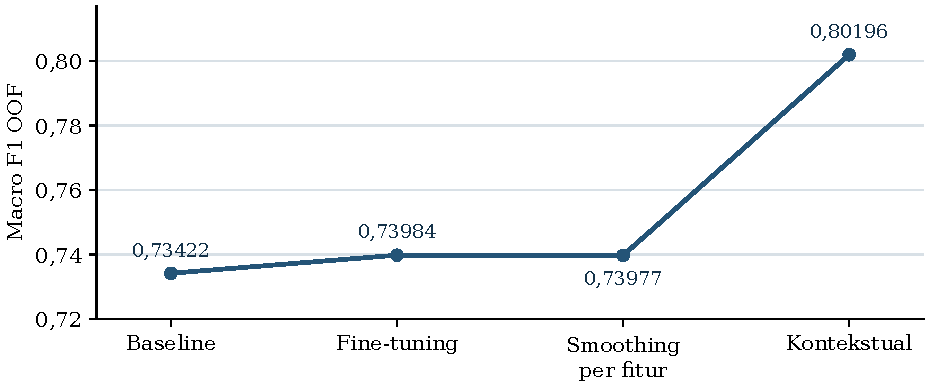
\includegraphics[width=0.84\textwidth]{nb_macro_f1.pdf}
\caption{Perubahan Macro F1 OOF antar-eksperimen pada protokol tim.}
\label{fig:nb_oof}
\end{figure}

Fine-tuning menaikkan Macro F1 sebesar 0,00562 dan memperbaiki empat dari lima fold. Dibanding baseline, false positive turun dari 3.917 ke 3.252, sedangkan false negative naik dari 2.688 ke 3.044. Smoothing per fitur menghasilkan perubahan total \(-0{,}00007\), walaupun tiga fold membaik tipis. Pada konfigurasi ini, smoothing yang lebih kuat untuk satu fitur belum menambah daya prediksi. Perubahan terbesar muncul pada tahap kontekstual, dengan kenaikan 0,06219 terhadap tahap sebelumnya. Karena tahap tersebut sekaligus mengubah diskretisasi, susunan fitur, dan pemilihan parameter, selisihnya mengukur efek gabungan.

\subsection{Validasi bertingkat dan perbandingan dengan scikit-learn}
Konfigurasi ekspor memperoleh OOF seleksi 0,80328 dengan threshold 0,45. Skor ini ikut menentukan konfigurasi yang dipilih. Validasi bertingkat memperoleh 0,79943 pada gabungan prediksi fold luar dan unggul pada lima fold terhadap \texttt{nb\_categorical\_tuned}, pembanding lama yang memakai bin hari rinci, kuantil tarif, dan gabungan kanal dengan rentang hari. Pembanding tersebut menggunakan prosedur validasi bertingkat yang sama dan berbeda dari baseline 17 fitur pada Tabel~\ref{tab:nb_tahap}.

\begin{table}[H]
\centering
\caption{Macro F1 pada fold luar validasi bertingkat kontekstual}
\label{tab:nb_nested}
\begin{tabular}{lrrr}
\toprule
Fold luar & Pembanding lama & Kontekstual & Threshold kontekstual \\
\midrule
1 & 0,75828 & 0,81082 & 0,435 \\
2 & 0,75328 & 0,79016 & 0,450 \\
3 & 0,75488 & 0,79297 & 0,475 \\
4 & 0,75433 & 0,80747 & 0,460 \\
5 & 0,74997 & 0,79571 & 0,420 \\
\midrule
OOF gabungan & 0,75421 & \textbf{0,79943} & -- \\
\bottomrule
\end{tabular}
\end{table}

\begin{table}[H]
\centering
\caption{Kesetaraan from scratch dengan pembanding scikit-learn pada konfigurasi yang sama}
\label{tab:nb}
\begin{tabularx}{\textwidth}{Xrrr}
\toprule
Tahap & From scratch & Pembanding & Selisih peluang maks. \\
\midrule
Baseline & 0,73422 & 0,73422 & \(6{,}00\times 10^{-15}\) \\
Fine-tuning (likelihood berbobot) & 0,73984 & 0,73984 & \(5{,}33\times 10^{-15}\) \\
Smoothing per fitur (likelihood berbobot) & 0,73977 & 0,73977 & \(5{,}44\times 10^{-15}\) \\
Kontekstual (OOF seleksi) & 0,80328 & 0,80328 & \(4{,}66\times 10^{-15}\) \\
\bottomrule
\end{tabularx}
\end{table}

Pada fine-tuning, \texttt{CategoricalNB} standar dengan bobot seragam dan \(\alpha=2\) memperoleh 0,73380. Pembanding berbobot memperoleh 0,73984. Selisih peluang pada Tabel~\ref{tab:nb} setara dengan galat pembulatan. Baris kontekstual memakai OOF seleksi karena verifikasi memakai konfigurasi ekspor dan fold yang sama.

\subsection{Analisis kesalahan, reproduksibilitas, dan bonus}
Prediksi gabungan fold luar kontekstual menghasilkan 15.960 \emph{true negative}, 2.444 \emph{false positive}, 2.400 \emph{false negative}, dan 6.569 \emph{true positive}. F1 kelas tidak batal mencapai 0,86824, sedangkan F1 kelas batal mencapai 0,73062. Pada kelompok \emph{lead time} lebih dari 80 hingga 151 hari, tingkat kesalahan masih 25,7\% dari 5.191 baris. Kelompok 11 hari atau kurang memiliki tingkat kesalahan 9,9\% dari 5.293 baris. Hasil ini menunjukkan bahwa kualitas prediksi berbeda antar-kelompok pemesanan setelah diskretisasi kontekstual.

Hasil run ulang \texttt{nb\_baseline} identik byte demi byte dengan \texttt{submission\_nb\_categorical\_all.csv} di branch \texttt{main}, yang mencatat public score 0,73697. Fine-tuning mencapai 0,74192 pada public leaderboard. Varian kontekstual mencapai 0,80173 dengan 6.844 prediksi dan threshold ekspor 0,45. Skor kontekstual 0,80196 dan 0,79943 berasal dari validasi data latih. KNN dengan vote booking kembar tetap menjadi model submission final kelompok.

Gambar~\ref{fig:nb_graf} menampilkan struktur dari sel bonus notebook kontekstual dengan label ringkas. Simpul \texttt{is\_canceled} memiliki sembilan anak sesuai masukan model. Panah menjelaskan faktorisasi peluang kondisional. Masing-masing simpul dapat berupa satu fitur atau satu kategori gabungan.

\begin{figure}[H]
\centering
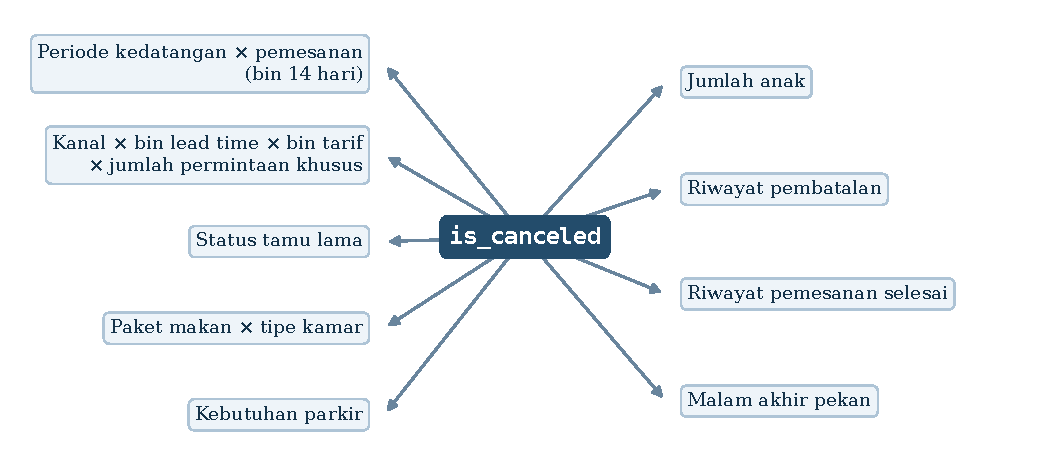
\includegraphics[width=\textwidth]{nb_graf.pdf}
\caption{Graf Bayesian Network untuk konfigurasi Categorical Naive Bayes kontekstual.}
\label{fig:nb_graf}
\end{figure}

\section{Kesimpulan}
Varian kontekstual mencapai Macro F1 OOF 0,80196 pada protokol tim dan 0,79943 pada validasi bertingkat. Skor public Kaggle varian ini adalah 0,80173. Pada preprocessing tetap, fine-tuning menghasilkan kenaikan kecil dan smoothing per fitur menghasilkan skor yang hampir sama. Pada data ini, perubahan representasi kategori memberi kenaikan yang lebih besar. Uji berikutnya dapat mengukur kontribusi diskretisasi kontekstual dan penggabungan kategori satu per satu pada fold luar yang sama.


\begingroup
\let\chapter\section
\small
\begin{thebibliography}{99}
\bibitem{ref:bayesnet} N. U. Maulidevi, “Bayes Net,” IF3170 Inteligensi Artifisial, Edunex ITB, 2024.
\bibitem{ref:categoricalnb} Scikit-learn developers, “Categorical Naive Bayes,” \emph{Scikit-learn User Guide}, bagian 1.9.5. \url{https://scikit-learn.org/stable/modules/naive_bayes.html#categorical-naive-bayes}

\bibitem{ref:zaidi_nb} N. A. Zaidi, J. Cerquides, M. J. Carman, dan G. I. Webb, “Alleviating Naive Bayes Attribute Independence Assumption by Attribute Weighting,” \emph{Journal of Machine Learning Research}, vol. 14, no. 60, hlm. 1947--1988, 2013. \url{https://www.jmlr.org/papers/v14/zaidi13a.html}

\bibitem{ref:fayyad_nb} U. M. Fayyad dan K. B. Irani, “Multi-Interval Discretization of Continuous-Valued Attributes for Classification Learning,” dalam \emph{Proc. IJCAI}, hlm. 1022--1028, 1993. \url{https://ijcai.org/proceedings/1993/141}

\bibitem{ref:pazzani_nb} M. J. Pazzani, “Searching for Dependencies in Bayesian Classifiers,” dalam \emph{Proc. Fifth International Workshop on Artificial Intelligence and Statistics}, hlm. 424--429, 1995. \url{https://proceedings.mlr.press/r0/pazzani95a.html}

\bibitem{ref:kohavi_nb} R. Kohavi dan G. H. John, “Wrappers for Feature Subset Selection,” \emph{Artificial Intelligence}, vol. 97, no. 1--2, hlm. 273--324, 1997. \url{https://doi.org/10.1016/S0004-3702(97)00043-X}

\end{thebibliography}
\endgroup

\else

% ---------------------------------------------------------------- sampul
\begin{titlepage}
  \centering
  {\large IF3170 Inteligensi Artifisial\par}
  \vspace{2.5cm}
  {\Huge\bfseries Tugas Besar 2\par}
  \vspace{0.5cm}
  {\LARGE Supervised Learning\par}
  \vspace{0.3cm}
  {\Large Prediksi Pembatalan Pemesanan Penginapan\par}
  \vspace{2.5cm}
  {\Large Kelompok 17 -- DerbyCounty\par}
  \vspace{1cm}
  \begin{tabular}{ll}
    13524032 & Juan Oloando Simanungkalit \\
    13524090 & Nashiruddin Akram \\
    13524093 & Reinsen Silitonga \\
    13524100 & Arghawisesa Dwinanda Arham \\
    13524102 & Manuel Thimoty Silalahi \\
  \end{tabular}
  \vfill
  {\large Program Studi Teknik Informatika\par}
  {\large Sekolah Teknik Elektro dan Informatika\par}
  {\large Institut Teknologi Bandung\par}
  {\large 2026\par}
\end{titlepage}

\pagenumbering{roman}
\tableofcontents
\listoffigures
\listoftables
\lstlistoflistings
\clearpage
\pagenumbering{arabic}

\chapter{Dasar Teori}

\section{Supervised Learning dan Klasifikasi Biner}
Supervised learning adalah pembelajaran mesin yang memakai data berlabel $D=\{(x_i,y_i)\}_{i=1}^{n}$ untuk mempelajari fungsi $h:X\rightarrow Y$ yang dapat memprediksi label data baru \cite{ref:intro}. Pada tugas ini $Y=\{0,1\}$, dengan $y=1$ berarti pemesanan dibatalkan (\texttt{is\_canceled}), sehingga persoalannya adalah klasifikasi biner. Semua model menghasilkan skor atau probabilitas $\hat{p}(x)=P(y=1\mid x)$, lalu label akhir diperoleh dengan ambang (threshold) $t$:
\begin{equation}
  \hat{y} = \mathbf{1}\left[\hat{p}(x) \geq t\right].
\end{equation}

\section{Tahapan Pengolahan Data}
Alur kerja mengikuti CRISP-DM \cite{ref:crispdm}: pemahaman bisnis, pemahaman data, persiapan data, pemodelan, evaluasi, dan deployment. Tahap persiapan data \cite{ref:dataprep} mencakup:
\begin{itemize}
  \item \textbf{Data cleaning}: menangani missing value, duplikat, outlier, dan nilai tidak valid.
  \item \textbf{Data transformation}: encoding kategori (misalnya one-hot), normalisasi atau standardisasi, serta penanganan data tidak seimbang.
  \item \textbf{Feature selection} dan \textbf{feature construction}: memilih fitur relevan dan membuat fitur turunan.
  \item \textbf{Dimensionality reduction}: memproyeksikan data ke dimensi lebih rendah bila jumlah fitur besar.
\end{itemize}
Seluruh statistik transformasi (batas clipping, median, modus, rata-rata, IQR, daftar kategori) harus dipelajari dari data latih saja, lalu diterapkan ke data validasi dan uji. Jika data validasi ikut dipakai saat fit, terjadi \emph{data leakage} dan skor validasi menjadi terlalu optimis.

\section{K-Nearest Neighbors (KNN)}
KNN adalah lazy learner \cite{ref:knn,ref:cunningham}. Tahap pelatihan hanya menyimpan data latih. Untuk query $q$, algoritma menghitung jarak ke seluruh data latih, mengambil $k$ tetangga terdekat $N_k(q)$, lalu melakukan voting. Jarak yang umum dipakai adalah jarak Minkowski orde $p$:
\begin{equation}
  d_p(q,x) = \Big(\sum_{j=1}^{m} |q_j - x_j|^{p}\Big)^{1/p},
\end{equation}
dengan $p=1$ sebagai jarak Manhattan dan $p=2$ sebagai jarak Euclidean. Probabilitas kelas 1 dengan voting seragam dan voting terbobot jarak berturut-turut adalah
\begin{equation}
  \hat{p}_{\text{uniform}}(q) = \frac{1}{k}\sum_{i\in N_k(q)} y_i, \qquad
  \hat{p}_{\text{weighted}}(q) = \frac{\sum_{i\in N_k(q)} w_i y_i}{\sum_{i\in N_k(q)} w_i}, \qquad w_i = \frac{1}{d(q,x_i)^2 + \epsilon}.
\end{equation}
Karena semua fitur berkontribusi pada jarak, KNN sangat sensitif terhadap skala fitur dan fitur yang tidak relevan. Pembobotan fitur, yaitu mengalikan kolom ke-$j$ dengan $w_j$ sebelum menghitung jarak, mengatur kontribusi tiap fitur \cite{ref:wettschereck}. Nilai $k$ kecil membuat model peka terhadap noise (variansi tinggi), sedangkan $k$ besar membuat prediksi condong ke kelas mayoritas (bias tinggi).

\section{Decision Tree Learning (DTL)}
Decision tree membagi ruang fitur secara rekursif berdasarkan atribut yang paling mengurangi ketidakmurnian (impurity) label \cite{ref:dtl03,ref:dtl04}. Untuk proporsi kelas positif $p$ pada suatu node:
\begin{align}
  \text{Entropy}(S) &= -p\log_2 p - (1-p)\log_2(1-p), \\
  \text{Gini}(S) &= 1 - p^2 - (1-p)^2 = 2p(1-p).
\end{align}
Information gain dari pemisahan $S$ menjadi $S_L$ dan $S_R$ adalah
\begin{equation}
  \text{Gain}(S) = I(S) - \frac{|S_L|}{|S|} I(S_L) - \frac{|S_R|}{|S|} I(S_R).
\end{equation}
Tiga varian algoritma yang dibahas di kuliah:
\begin{itemize}
  \item \textbf{ID3}: memakai entropi dan information gain, dengan cabang sebanyak nilai atribut kategorikal.
  \item \textbf{C4.5}: memakai gain ratio, mendukung atribut kontinu melalui threshold, menangani missing value, dan melakukan post-pruning \cite{ref:quinlan}. Gain ratio menormalkan gain dengan split information:
  \begin{equation}
    \text{GainRatio}(S) = \frac{\text{Gain}(S)}{\text{SplitInfo}(S)}, \qquad
    \text{SplitInfo}(S) = -\sum_{v\in\{L,R\}} \frac{|S_v|}{|S|}\log_2\frac{|S_v|}{|S|}.
  \end{equation}
  \item \textbf{CART}: pohon biner dengan Gini, atribut kontinu dipotong di titik tengah dua nilai berurutan, dan dapat dipangkas dengan cost-complexity pruning \cite{ref:breiman}.
\end{itemize}
Atribut kontinu ditangani dengan mengurutkan nilai lalu mencoba setiap titik potong di antara dua nilai berbeda \cite{ref:dtlcont}. Missing value dapat ditangani dengan mengarahkan baris kosong ke cabang yang paling menguntungkan \cite{ref:dtlmiss}. Overfitting dicegah dengan pre-pruning (batas kedalaman, jumlah minimum sampel per daun, minimum gain) atau post-pruning \cite{ref:dtloverfit}.

\section{Logistic Regression}
Logistic regression memodelkan probabilitas kelas positif dengan fungsi sigmoid dari kombinasi linear fitur \cite{ref:lrwhat}:
\begin{equation}
  \hat{p}(x) = \sigma(\theta^\top x + b), \qquad \sigma(z) = \frac{1}{1+e^{-z}}.
\end{equation}
Parameter dipelajari dengan meminimalkan log-loss ditambah suku regularisasi $R(\theta)$:
\begin{equation}
  J(\theta) = -\frac{1}{n}\sum_{i=1}^{n}\left[y_i\log\hat{p}_i + (1-y_i)\log(1-\hat{p}_i)\right] + \lambda R(\theta).
\end{equation}
Gradien log-loss adalah $\nabla_\theta = \frac{1}{n}X^\top(\hat{p}-y)$, sehingga parameter dapat diperbarui dengan gradient descent \cite{ref:lrsga}. Tiga bentuk regularisasi yang diminta spesifikasi adalah L1 ($R=\lVert\theta\rVert_1$, mendorong sebagian bobot menjadi tepat nol), L2 ($R=\frac{1}{2}\lVert\theta\rVert_2^2$, mengecilkan bobot secara halus), dan Elastic Net ($R=\alpha\lVert\theta\rVert_1 + \frac{1-\alpha}{2}\lVert\theta\rVert_2^2$).

\section{Support Vector Machine (SVM)}
SVM mencari hyperplane $w^\top x + b = 0$ dengan margin terbesar antara dua kelas \cite{ref:svmwhat,ref:svmsep}. Dengan label $y_i\in\{-1,+1\}$, formulasi soft margin untuk data yang tidak terpisah linear \cite{ref:svmnonsep} adalah
\begin{equation}
  \min_{w,b,\xi}\ \frac{1}{2}\lVert w\rVert^2 + C\sum_i \xi_i \quad \text{s.t.}\quad y_i(w^\top x_i + b)\ge 1-\xi_i,\ \xi_i\ge 0.
\end{equation}
Bentuk dual-nya hanya bergantung pada hasil kali dalam antardata, sehingga dapat diganti dengan fungsi kernel $K(x_i,x_j)$:
\begin{equation}
  \min_\alpha\ \frac{1}{2}\sum_{i,j}\alpha_i\alpha_j y_i y_j K(x_i,x_j) - \sum_i\alpha_i \quad \text{s.t.}\quad 0\le\alpha_i\le C,\ \sum_i\alpha_i y_i = 0.
\end{equation}
Kernel yang diimplementasikan adalah linear $K(x,z)=x^\top z$, polynomial $K(x,z)=(\gamma x^\top z + r)^d$, dan Gaussian $K(x,z)=\exp(-\gamma\lVert x-z\rVert^2)$. Untuk $n$ besar, masalah dual diselesaikan dengan dekomposisi working set \cite{ref:platt_smo,ref:fan}. Probabilitas diperoleh dengan Platt scaling \cite{ref:platt_prob}.

\section{Naive Bayes}
Naive Bayes menerapkan teorema Bayes dengan asumsi setiap fitur saling independen bersyarat terhadap kelas \cite{ref:bayesnet}. Asumsi ini setara dengan Bayesian network berbentuk bintang dengan kelas sebagai satu-satunya induk semua fitur:
\begin{equation}
  P(y\mid x) \propto P(y)\prod_{j=1}^{m} P(x_j\mid y).
\end{equation}
Untuk fitur kategorikal, peluang bersyarat diestimasi dengan Laplace smoothing $P(x_j=v\mid y=c)=\frac{N_{j,v,c}+\alpha}{N_c+\alpha V_j}$, dan perhitungan dilakukan dalam ruang logaritma agar tidak terjadi underflow.

\section{Evaluasi Model}
Untuk klasifikasi biner, confusion matrix terdiri atas TN, FP, FN, dan TP. Untuk tiap kelas $c$:
\begin{equation}
  \text{Precision}_c = \frac{TP_c}{TP_c+FP_c},\qquad \text{Recall}_c = \frac{TP_c}{TP_c+FN_c},\qquad F1_c = \frac{2\,TP_c}{2\,TP_c+FP_c+FN_c}.
\end{equation}
Metrik kompetisi adalah \textbf{Macro F1}, yaitu rata-rata $F1$ kelas 0 dan kelas 1. Metrik ini memberi bobot sama pada kedua kelas, sehingga lebih tepat daripada akurasi untuk data yang tidak seimbang.

Stratified $k$-fold cross validation membagi data menjadi $k$ bagian dengan proporsi kelas yang sama. Gabungan prediksi pada data validasi tiap fold disebut prediksi \textbf{out-of-fold (OOF)}. Setiap baris latih memperoleh tepat satu prediksi dari model yang tidak pernah melihat baris tersebut, sehingga OOF dapat dipakai untuk memilih hyperparameter dan threshold tanpa menyentuh data uji.

\chapter{Implementasi}

\section{Deskripsi Persoalan dan Pemahaman Data}
Sebuah penginapan ingin memperkirakan pemesanan yang akan dibatalkan agar perencanaan kamar, overbooking, dan kebijakan pembatalan lebih akurat. Dataset Kaggle terdiri atas \texttt{train.csv} (27.373 baris, 17 fitur, dan target) dan \texttt{test.csv} (6.844 baris). Prediksi dinilai dengan Macro F1.

\begin{table}[H]
\centering
\caption{Fitur pada dataset}
\label{tab:fitur}
\begin{tabularx}{\textwidth}{>{\ttfamily\raggedright\arraybackslash}p{6.2cm}X}
\toprule
\normalfont\textbf{Fitur} & \textbf{Keterangan} \\
\midrule
num\_adults, num\_children & Jumlah tamu dewasa dan anak \\
weekend\_nights, weekday\_nights & Jumlah malam akhir pekan dan hari kerja \\
meal\_package & Paket makan (kategorikal) \\
needs\_parking & 1 jika membutuhkan parkir \\
room\_category & Kategori kamar Type A sampai G (kategorikal, tidak berurutan) \\
days\_before\_arrival & Selisih hari antara pemesanan dan kedatangan (lead time) \\
arrival\_year/month/day & Tanggal kedatangan \\
booking\_channel & Kanal pemesanan (kategorikal) \\
is\_returning\_guest & 1 jika tamu pernah menginap \\
prior\_cancellations, prior\_completed\_bookings & Riwayat pemesanan tamu \\
nightly\_rate\_idr & Harga rata-rata per malam (IDR) \\
special\_requests & Jumlah permintaan khusus \\
is\_canceled & Target (1 = batal) \\
\bottomrule
\end{tabularx}
\end{table}

Temuan utama dari eksplorasi data (bagian Data Understanding pada \texttt{src/main.ipynb}):
\begin{itemize}
  \item \textbf{Ketidakseimbangan kelas}: 67,2\% tidak batal dan 32,8\% batal (sekitar 2:1), tidak seimbang tetapi tidak ekstrem.
  \item \textbf{Missing value} pada delapan kolom, antara 3\% dan 11\% (Tabel~\ref{tab:missing}), dengan proporsi hampir sama di train dan test. Rasio batal baris kosong dan terisi hanya berbeda di bawah 2 poin persen, kecuali \texttt{special\_requests} (40,8\% jika kosong, 32,0\% jika terisi).
  \item \textbf{Duplikat dan nilai janggal}: 64 baris duplikat persis (fitur dan target), 106 pemesanan tanpa tamu dewasa, 64 pemesanan dengan total malam 0, 3 pemesanan dengan 9 atau 10 anak, dan 146 pemesanan berharga 0 di luar kanal Complimentary.
  \item \textbf{Skala fitur} sangat berbeda: \texttt{nightly\_rate\_idr} berada pada 0 sampai Rp9.165.000, sedangkan fitur biner hanya 0 sampai 1. Lead time sangat menceng ke kanan (median 58 hari, maksimum 448 hari).
  \item \textbf{Sinyal terkuat}: \texttt{days\_before\_arrival} (korelasi 0,44 dengan target, rasio batal naik dari 8,8\% pada lead time 0 sampai 5 hari menjadi 73,8\% di atas 192 hari), \texttt{special\_requests} ($-0{,}26$; 43,2\% batal tanpa permintaan khusus dan hampir tidak ada pembatalan pada 3 permintaan atau lebih), dan kanal pemesanan (Complimentary 0\%, Corporate 11,5\%, Online Travel Agent 36,4\%).
  \item \textbf{Pola musiman}: rasio batal terendah pada Januari (2,6\%) dan Desember (12,1\%), tertinggi pada Juli (44,8\%). Korelasi linear \texttt{arrival\_month} hampir nol ($-0{,}016$) karena polanya naik lalu turun, sehingga perlu encoding melingkar.
\end{itemize}

\begin{table}[H]
\centering
\caption{Persentase missing value pada train dan test}
\label{tab:missing}
\begin{tabular}{lrr}
\toprule
Kolom & Train (\%) & Test (\%) \\
\midrule
num\_children & 11,09 & 10,91 \\
special\_requests & 9,13 & 8,66 \\
nightly\_rate\_idr & 7,45 & 7,89 \\
meal\_package & 6,43 & 6,46 \\
days\_before\_arrival & 4,10 & 4,24 \\
needs\_parking & 3,95 & 3,61 \\
room\_category & 3,66 & 3,54 \\
num\_adults & 2,96 & 2,63 \\
\bottomrule
\end{tabular}
\end{table}

\begin{figure}[H]
\centering
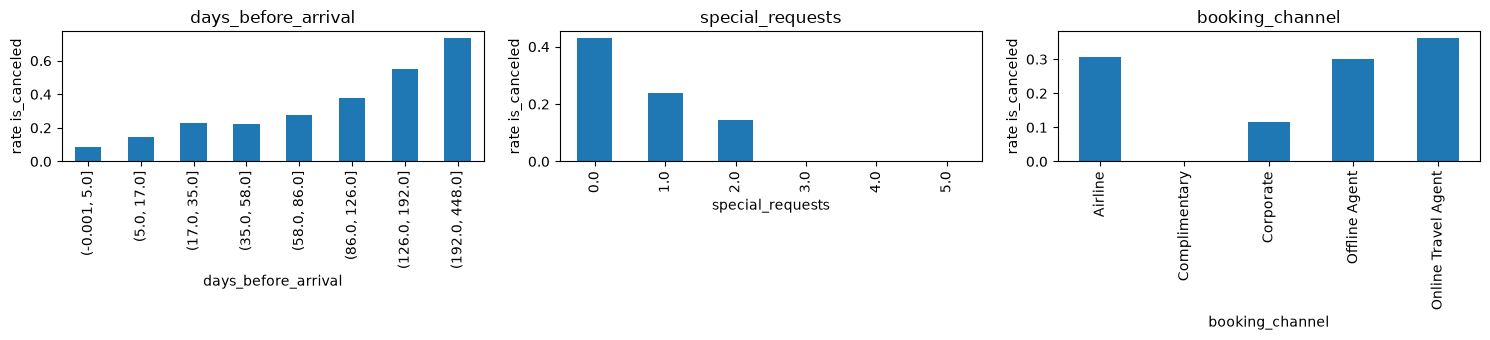
\includegraphics[width=\textwidth]{eda_target_rate.png}
\caption{Rasio batal per lead time, jumlah permintaan khusus, dan kanal pemesanan}
\label{fig:eda_rate}
\end{figure}

\begin{figure}[H]
\centering
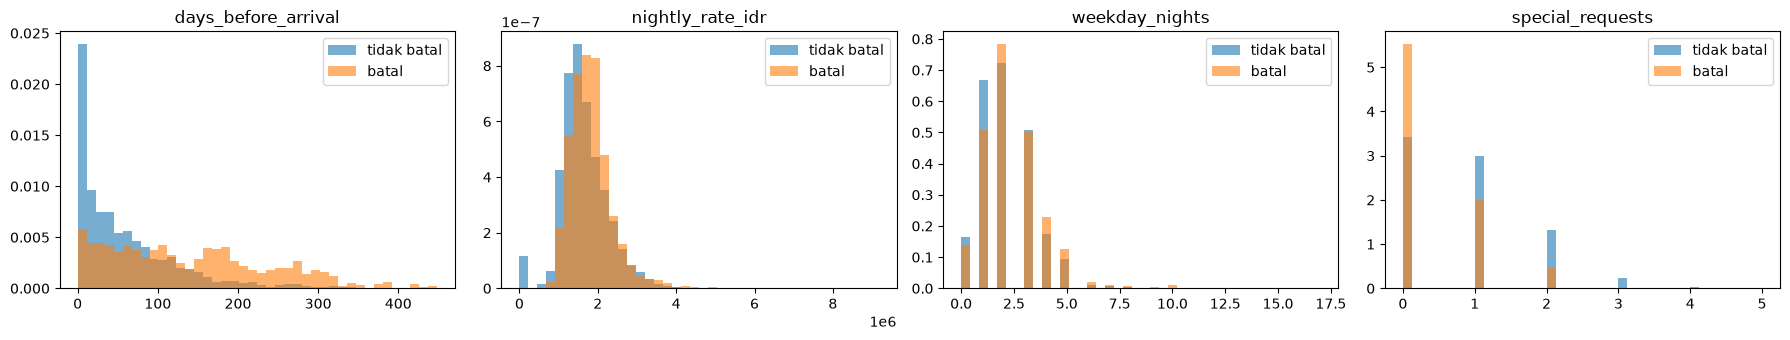
\includegraphics[width=\textwidth]{eda_histogram.png}
\caption{Distribusi fitur numerik per kelas (density)}
\label{fig:eda_hist}
\end{figure}

\begin{figure}[H]
\centering
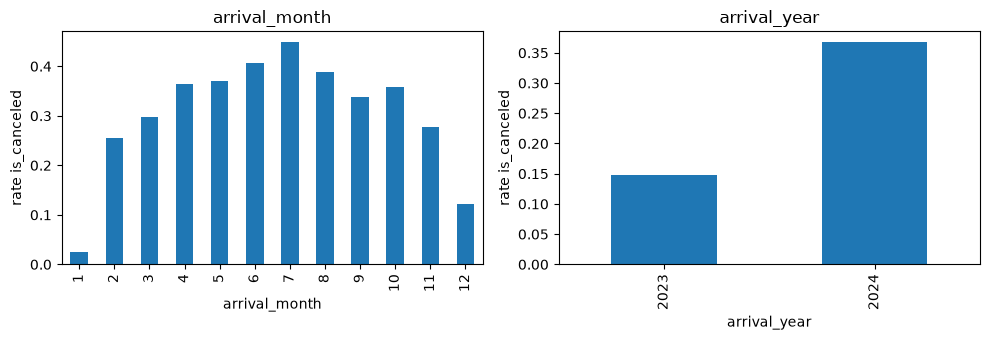
\includegraphics[width=0.8\textwidth]{eda_musim.png}
\caption{Rasio batal per bulan dan tahun kedatangan}
\label{fig:eda_musim}
\end{figure}

\begin{figure}[H]
\centering
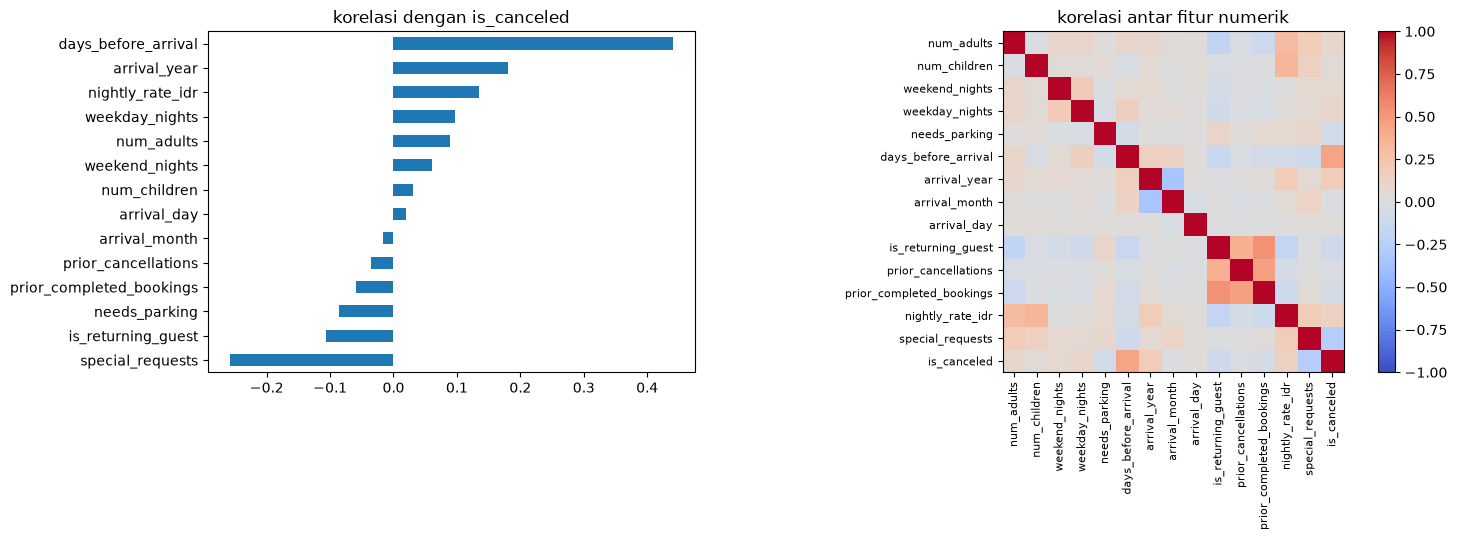
\includegraphics[width=\textwidth]{eda_korelasi.png}
\caption{Korelasi fitur numerik dengan target (kiri) dan antarfitur (kanan)}
\label{fig:eda_korelasi}
\end{figure}

\paragraph{Booking kembar dan noise.} Data ini diberi noise oleh penyelenggara. Untuk melihat kolom mana yang diberi noise, dicari pasangan pemesanan yang identik di semua kolom kecuali lead time dan tanggal datang. Dari 176 pasangan yang berdekatan, 93,2\% memiliki label yang sama. Tanggal datang hampir selalu sama (91,5\% berbeda paling banyak 1 hari, simpangan baku 1,98 hari), sedangkan lead time menyebar (hanya 25\% berbeda paling banyak 1 hari, simpangan baku 4,78 hari). Temuan ini menjadi dasar vote booking kembar pada model KNN final (Bagian~\ref{sec:knn}).

\begin{figure}[H]
\centering
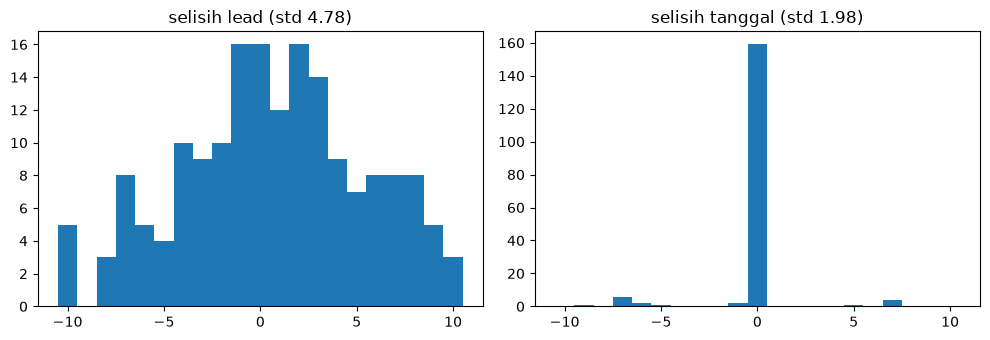
\includegraphics[width=0.8\textwidth]{eda_kembar.png}
\caption{Selisih lead time dan tanggal datang pada pasangan booking identik}
\label{fig:eda_kembar}
\end{figure}

\section{Struktur Program}
Seluruh kode from scratch (preprocessing, model, dan validasi) ditulis langsung di dalam notebook, tanpa modul Python terpisah. Format notebook mengikuti templat tugas.
\begin{itemize}
  \item \texttt{src/main.ipynb}: notebook final yang mereproduksi submission Kaggle. Berisi pemahaman data, preprocessing bersama, model KNN final, Decision Tree terbaik, perbandingan scikit-learn, save/load model, submission, error analysis, dan cost-sensitive classification.
  \item \texttt{src/experiments/<model>/}: notebook eksperimen tiap model (\texttt{knn}, \texttt{dtl}, \texttt{lr}, \texttt{svm}, \texttt{nb}). Satu notebook untuk satu eksperimen.
  \item \texttt{output/submissions/}: berkas submission; \texttt{output/models/}: model tersimpan (\texttt{.pkl}); \texttt{output/figures/}: gambar dan video untuk bonus.
\end{itemize}
Setiap model mengikuti antarmuka yang sama: \texttt{fit(X, y)}, \texttt{predict\_proba(X)} yang mengembalikan probabilitas kelas 1, dan \texttt{predict(X, threshold)}. Setiap notebook mencetak md5 berkas submission di akhir untuk membuktikan bahwa hasilnya reproducible.

\section{Data Cleaning dan Preprocessing}

\subsection{Preprocessing bersama}
Preprocessing bersama dipakai oleh KNN final dan Logistic Regression (notebook \texttt{lr\_main\_*}). Setiap langkah ditulis sebagai fungsi kecil yang menerima list \texttt{frames}, mengambil statistik dari \texttt{frames[0]} (data fit), lalu menerapkannya ke semua frame. Fungsi \texttt{prepare} menggabungkan semua langkah dengan urutan yang benar.

\begin{table}[H]
\centering
\caption{Langkah preprocessing bersama beserta alasannya}
\label{tab:prep_bersama}
\begin{tabularx}{\textwidth}{>{\raggedright\arraybackslash}p{3.3cm}>{\raggedright\arraybackslash}p{4.7cm}X}
\toprule
Langkah & Transformasi & Alasan \\
\midrule
Dedupe & Buang 64 baris duplikat (fitur dan target) sebelum split & Duplikat bisa berada di fold latih dan validasi sekaligus sehingga skor terlalu optimis \\
Data error & \texttt{num\_adults = 0} menjadi missing & Pemesanan tanpa tamu dewasa tidak masuk akal \\
Outlier & Clipping ke persentil 0,5\% dan 99,5\% data fit & Nilai ekstrem tidak mendominasi jarak \\
Fitur turunan & \texttt{booking\_index} (tanggal booking) dan \texttt{month\_cos} (musim) & Lead time dan tanggal datang digabung, Desember dan Januari berdekatan \\
Imputasi & Median (numerik), modus (kategorikal) dari data fit & Lebih baik dari mean, modus, KNN imputation, group median, dan jarak yang mengabaikan missing \\
Scaling & Robust scaler $(x-\text{median})/\text{IQR}$ & Tidak terpengaruh outlier, lebih baik dari z-score, min-max, dan rank \\
Bobot fitur & Lead time dan special\_requests $\times2$, needs\_parking dan weekday\_nights $\times0{,}5$, num\_adults $\times0{,}25$ & Hasil coordinate search, menekankan fitur yang paling informatif \\
Encoding & One-hot dengan nilai 0,75 & Kategori tidak berurutan, nilai 0,75 agar beda kategori tidak terlalu dominan \\
\bottomrule
\end{tabularx}
\end{table}

Hasilnya 15 fitur atau 28 kolom (12 numerik dan 16 one-hot). Reduksi dimensi dilakukan dengan seleksi fitur (forward selection), bukan PCA, agar fitur tetap dapat dijelaskan dan diberi bobot sendiri-sendiri. Ketidakseimbangan kelas tidak ditangani dengan resampling, tetapi dengan memilih threshold yang memaksimalkan Macro F1.

\begin{lstlisting}[caption={Pipeline preprocessing bersama (\texttt{src/main.ipynb})}, label={lst:prepare}]
def prepare(fit_df, *dfs):
    frames = [df.copy() for df in (fit_df,) + dfs]
    mark_invalid(frames)                                  # num_adults = 0 -> NaN
    cap_outliers(frames, clip_col, CFG.CLIP_QUANTILE)     # persentil 0.5% dan 99.5%
    engineer(frames)                                      # booking_index, month_cos
    impute(frames, num_col, 'median')
    impute(frames, cat_col, 'most_frequent')
    scale(frames, num_col)                                # robust scaler
    weight(frames, CFG.FEATURE_WEIGHTS)
    columns = num_col + encode(frames, cat_col, CFG.ONEHOT_VALUE)
    return [frame[columns].to_numpy(np.float32) for frame in frames]

def cap_outliers(frames, columns, q=0.005):
    lower, upper = frames[0][columns].quantile(q), frames[0][columns].quantile(1 - q)
    same = lower >= upper
    lower, upper = lower.where(~same, -np.inf), upper.where(~same, np.inf)
    for frame in frames:
        frame[columns] = frame[columns].clip(lower, upper, axis=1)

def scale(frames, columns):
    fit = frames[0][columns].astype(float)
    center = fit.median()
    spread = fit.quantile(0.75) - fit.quantile(0.25)
    spread = spread.where(spread > 0, fit.std()).replace(0, 1)
    for frame in frames:
        frame[columns] = (frame[columns].astype(float) - center) / spread
\end{lstlisting}

\subsection{Preprocessing khusus model}
Setiap algoritma memiliki asumsi berbeda terhadap bentuk data, sehingga sebagian eksperimen memakai preprocessing sendiri (Tabel~\ref{tab:prep_model}).

\begin{table}[H]
\centering
\caption{Preprocessing khusus model beserta alasannya}
\label{tab:prep_model}
\begin{tabularx}{\textwidth}{>{\raggedright\arraybackslash}p{2.4cm}>{\raggedright\arraybackslash}p{5.6cm}X}
\toprule
Model & Transformasi & Alasan \\
\midrule
DTL & Dedupe, \texttt{num\_adults = 0} jadi missing, 7 fitur turunan, kategori langka ($<20$ baris) menjadi \texttt{Other}. NaN dan kategori teks dibiarkan, tanpa scaling & Pohon menangani missing dan kategori langsung. Split berbasis urutan nilai sehingga tidak terpengaruh skala \\
LR & Indikator missing, imputasi median, \texttt{log1p}, encoding siklik, one-hot, binning berbasis target, interaksi fitur & Model linear butuh representasi yang menangkap hubungan tidak linear dan interaksi \\
SVM & Imputasi, one-hot, standardisasi, ditambah fitur turunan & Kernel dihitung dari hasil kali dalam atau jarak sehingga sensitif terhadap skala \\
NB & Setiap fitur menjadi kode kategori; lead time dikelompokkan ke $\le30$, 30 sampai 90, dan $>90$ hari; tarif ke $\le1$ juta, 1 sampai 2 juta, dan $>2$ juta. Nilai kosong menjadi kategori sendiri & Categorical Naive Bayes membutuhkan nilai diskrit \\
\bottomrule
\end{tabularx}
\end{table}

Tujuh fitur turunan pada DTL adalah \texttt{total\_nights}, \texttt{total\_guests}, \texttt{is\_free} (harga 0), \texttt{rate\_per\_guest}, \texttt{arrival\_weekday}, \texttt{arrival\_dayofyear}, dan \texttt{arrival\_index} (hari sejak 1 Januari 2023).

\begin{lstlisting}[caption={Preprocessing DTL (\texttt{src/experiments/dtl/})}, label={lst:prepare_tree}]
def group_rare(frames, columns, min_count=20):
    for column in columns:
        counts = frames[0][column].value_counts()
        keep = sorted(counts[counts >= min_count].index)
        for frame in frames:
            known = frame[column].isin(keep) | frame[column].isna()
            frame.loc[~known, column] = 'Other'

def prepare_tree(fit_df, *dfs):
    frames = [df.copy() for df in (fit_df,) + dfs]
    mark_invalid(frames)
    add_features(frames)
    frames = [f.drop(columns=[c for c in [ID, TARGET] if c in f.columns]) for f in frames]
    group_rare(frames, cat_col, CFG.RARE_MIN_COUNT)
    return frames          # NaN dan kategori teks dibiarkan untuk pohon
\end{lstlisting}

\section{Skema Validasi}
Semua preprocessing di-fit ulang di setiap fold hanya dengan data latih fold tersebut. Threshold dipilih dari grid 0,20 sampai 0,80 dengan langkah 0,01 berdasarkan Macro F1 OOF.
\begin{itemize}
  \item \textbf{Notebook final}: holdout 20\% stratified (seed 5) untuk membandingkan model, dan 5-fold OOF untuk skor akhir.
  \item \textbf{Eksperimen}: stratified 5-fold manual dengan seed 42. Setiap perubahan dicek ulang pada beberapa seed fold lain (seed 1 sampai 5 untuk DTL, seed 4, 5, dan 42 untuk KNN) agar kenaikan tidak hanya kebetulan dari satu pembagian data.
\end{itemize}
Model final dilatih ulang pada seluruh data latih, disimpan dengan \texttt{pickle}, lalu dimuat ulang untuk membuat submission.

\section{K-Nearest Neighbors}
\label{sec:knn}
Kelas \texttt{KNN} hanya memakai NumPy. Jarak Minkowski dijumlah per kolom dalam float32 agar memori cukup, lalu $k$ tetangga terdekat dipilih dengan \texttt{argpartition} dan diurutkan secara stabil. Model final memakai $k=17$, $p=1{,}5$, dan bobot vote $1/(d^2+10^{-6})$.

\begin{lstlisting}[caption={Kelas KNN (\texttt{src/main.ipynb})}, label={lst:knn}]
class KNN:
    def __init__(self, k=5, p=2.0, batch=1024):
        self.k, self.p, self.batch = k, p, batch

    def fit(self, X, y):
        self.X, self.y = X, np.asarray(y).astype(int)
        return self

    def kneighbors(self, Q):
        dists, ids = [], []
        for start in range(0, len(Q), self.batch):
            q = Q[start:start + self.batch]
            D = np.zeros((len(q), len(self.X)), np.float32)
            for j in range(self.X.shape[1]):
                D += np.abs(q[:, j, None] - self.X[None, :, j]) ** self.p
            idx = np.argpartition(D, self.k - 1, axis=1)[:, :self.k]
            d = np.take_along_axis(D, idx, 1)
            order = np.argsort(d, axis=1, kind='stable')
            ids.append(np.take_along_axis(idx, order, 1))
            dists.append(np.take_along_axis(d, order, 1) ** (1 / self.p))
        return np.vstack(dists), np.vstack(ids)

    def predict_proba(self, Q):
        d, idx = self.kneighbors(Q)
        w = 1 / (d ** 2 + 1e-6)
        return (w * self.y[idx]).sum(1) / w.sum(1)
\end{lstlisting}

\paragraph{Vote booking kembar.} Berdasarkan temuan noise pada lead time, KNN final digabung dengan vote dari \emph{booking kembar}: baris latih dengan kolom \texttt{twin\_key} (jumlah malam, kanal, status tamu, riwayat pemesanan) sama persis, kolom \texttt{twin\_soft} (jumlah tamu, parkir, paket makan, kamar, permintaan khusus) sama atau kosong, selisih lead time paling banyak 10 hari, selisih tanggal datang paling banyak 2 hari, dan selisih harga paling banyak 6\%. Jika ada minimal 2 kembar, probabilitas akhir adalah
\begin{equation}
  \hat{p} = 0{,}2\,\hat{p}_{\text{KNN}} + 0{,}8\,\frac{\text{jumlah kembar yang batal}}{\text{jumlah kembar}},
\end{equation}
dan label batal diberikan jika $\hat{p}\ge0{,}4845$. Toleransi lead time dibuat longgar dan toleransi tanggal datang dibuat ketat karena noise terutama ada pada lead time.

\begin{lstlisting}[caption={Vote booking kembar (diringkas)}, label={lst:twin}]
def twin_vote(A, B, y_B, lead, day, price):
    groups_b = B.groupby(twin_key, dropna=False).indices
    for key, ia in A.groupby(twin_key, dropna=False).indices.items():
        ib = groups_b.get(key)                 # kolom kunci harus sama persis
        if ib is None:
            continue
        a, b = A.iloc[ia], B.iloc[ib]
        ok = np.ones((len(ia), len(ib)), bool)
        for c in twin_soft:                    # sama, atau salah satunya kosong
            x, z = a[c].to_numpy()[:, None], b[c].to_numpy()[None, :]
            ok &= (x == z) | pd.isna(x) | pd.isna(z)
        ok &= abs_diff(a, b, 'days_before_arrival') <= lead
        ok &= date_diff(a, b) <= day
        ok &= rel_diff(a, b, 'nightly_rate_idr') <= price
        n = ok.sum(1)
        share[ia] = (ok * y_B[ib][None, :]).sum(1) / np.maximum(n, 1)
        count[ia] = n
    return share, count
\end{lstlisting}

\section{Decision Tree Learning (C4.5)}
Kelas \texttt{DecisionTree} mengimplementasikan pohon biner dengan pilihan criterion gini, entropy, atau gain ratio. Model terbaik memakai \textbf{gain ratio (C4.5)} dengan split biner. Implementasi ini menangani tiga jenis data yang diminta spesifikasi secara langsung:
\begin{itemize}
  \item \textbf{Numerik}: nilai diurutkan, lalu jumlah kumulatif label positif dipakai untuk menghitung impurity semua titik potong sekaligus. Threshold adalah titik tengah dua nilai berbeda yang berurutan.
  \item \textbf{Kategorikal}: kolom bertipe teks dikenali otomatis. Kategori diurutkan berdasarkan proporsi kelas positif, lalu dicari titik potong terbaik di antara peringkatnya, sehingga cukup mencoba $c-1$ titik potong.
  \item \textbf{Missing value}: split dicari dari baris yang terisi. Kedua kemungkinan (baris kosong ke kiri atau ke kanan) dievaluasi, dan arah dengan impurity terkecil disimpan sebagai arah default untuk prediksi. Kategori yang tidak dikenal saat prediksi juga mengikuti arah ini.
\end{itemize}
Sesuai C4.5, gain ratio hanya dihitung untuk split yang information gain-nya minimal sebesar rata-rata gain, agar split dengan split information sangat kecil tidak terpilih.

\begin{lstlisting}[caption={Pemilihan split dengan gain ratio (diringkas)}, label={lst:gainratio}]
if self.criterion == 'gain_ratio':
    # C4.5: gain ratio hanya untuk split point dengan gain >= rata-rata gain
    ok = gain > 1e-12
    if not ok.any():
        continue
    ok &= gain >= gain[ok].mean() - 1e-12
    split_info = _impurity(nl, np.full_like(nl, split_total), 'entropy')
    ratio = np.where(ok, gain / np.maximum(split_info, 1e-12), -np.inf)
    i = int(np.argmax(ratio))
    candidates.append((float(ratio[i]), make_split(i, float(gain[i]))))
\end{lstlisting}

Pre-pruning dilakukan dengan \texttt{max\_depth}, \texttt{min\_samples\_leaf}, dan \texttt{min\_impurity\_decrease} (minimum gain). Konfigurasi terbaik adalah gain ratio dengan \texttt{max\_depth} 30, \texttt{min\_samples\_leaf} 5, dan \texttt{min\_impurity\_decrease} $2\times10^{-4}$, dipilih dengan grid search yang memilih sel dengan rata-rata skor tetangga tertinggi agar tidak memilih puncak yang sempit.

\paragraph{Cost-complexity pruning.} Sebagai algoritma optimasi di luar materi kuliah (materi hanya membahas reduced-error pruning dan rule post-pruning), pohon dapat dipangkas setelah dibangun dengan cost-complexity pruning \cite{ref:breiman}:
\begin{equation}
  R_\alpha(T) = R(T) + \alpha\,|\tilde{T}|,
\end{equation}
dengan $R(T)$ jumlah impurity leaf yang dibobot proporsi sampel dan $|\tilde{T}|$ jumlah leaf. Sebuah node dijadikan leaf jika $R(\text{node})+\alpha \le R(\text{subtree})+\alpha\,|\tilde{T}_{\text{subtree}}|$.

\begin{lstlisting}[caption={Cost-complexity pruning}, label={lst:ccp}]
def cost_complexity_prune(self, alpha):
    crit = 'gini' if self.criterion == 'gini' else 'entropy'
    def visit(node):
        r_leaf = node.n_samples / self.n_total_ * float(_impurity(node.n_pos, node.n_samples, crit))
        if node.is_leaf:
            return r_leaf, 1
        r_left, n_left = visit(node.left)
        r_right, n_right = visit(node.right)
        r_sub, n_sub = r_left + r_right, n_left + n_right
        if r_leaf + alpha <= r_sub + alpha * n_sub:    # subtree tidak sebanding dengan leaf-nya
            node.left = node.right = None
            node.feature = None
            return r_leaf, 1
        return r_sub, n_sub
    visit(self.root_)
    return self
\end{lstlisting}

\section{Logistic Regression}
Kelas \texttt{LogisticRegression} meminimalkan log-loss dengan regularisasi L1, L2, atau Elastic Net. Bagian L2 masuk ke gradien, sedangkan bagian L1 yang tidak terdiferensiasi di nol ditangani dengan proximal step (soft-thresholding) sehingga bobot yang tidak penting benar-benar bernilai nol. Selain gradient descent biasa, tersedia solver \textbf{FISTA} \cite{ref:fista}: gradien dihitung di titik momentum Nesterov, ukuran langkah $1/L$ dihitung dari konstanta Lipschitz, dan momentum di-reset ketika arah langkah berbalik (adaptive restart).

\begin{lstlisting}[caption={Satu iterasi FISTA dengan proximal step L1 (diringkas)}, label={lst:fista}]
err = s * (sigmoid(zv) - y) / S
w_new = wv - lr * (X.T @ err + lam2 * wv)          # gradien log-loss + L2
b_new = bv - lr * float(err.sum())
if lam1 > 0:                                       # proximal step untuk L1
    w_new = xp.sign(w_new) * xp.maximum(xp.abs(w_new) - lr * lam1, 0.0)
if self.solver == 'fista':
    if float((wv - w_new) @ (w_new - w)) + (bv - b_new) * (b_new - b) > 0:
        t = 1.0                                    # adaptive restart
    t_next = (1.0 + np.sqrt(1.0 + 4.0 * t * t)) / 2.0
    beta = (t - 1.0) / t_next
    t = t_next
wv = w_new + beta * (w_new - w)                    # titik momentum Nesterov
bv = b_new + beta * (b_new - b)
\end{lstlisting}

Tuning dilakukan dalam empat tahap preprocessing khusus model linear (\texttt{lr\_fe}, \texttt{lr\_target\_bins}, \texttt{lr\_l1\_onehot}, \texttt{lr\_cross\_bins}), ditambah dua notebook yang memakai preprocessing bersama (\texttt{lr\_main\_prep} dan \texttt{lr\_main\_expand}).

\section{Support Vector Machine}
Kelas \texttt{SVM} menyelesaikan bentuk dual untuk kernel linear, polynomial, dan Gaussian. Subproblem QP diselesaikan dengan SLSQP dalam blok working set berisi paling banyak 64 variabel alpha, sehingga matriks kernel penuh tidak perlu disimpan. Fungsi keputusan $f(x)=\sum_{i\in SV}\alpha_i y_i K(x_i,x)+b$ dikalibrasi menjadi probabilitas dengan Platt scaling menggunakan holdout internal 20\%. Hyperparameter $C$ dan $\gamma$ dicari dengan \textbf{Particle Swarm Optimization (PSO)} \cite{ref:pso,ref:pso_shi}: setiap partikel adalah kandidat $(\log_{10}C, \log_{10}g)$, dan posisinya diperbarui dengan
\begin{equation}
  v_i \leftarrow w v_i + c_1 r_1 (p_i - x_i) + c_2 r_2 (g^{*} - x_i), \qquad x_i \leftarrow x_i + v_i,
\end{equation}
dengan fitness berupa Macro F1 OOF. \todo{Akram: lengkapi detail implementasi dan hasil PSO dari notebook \texttt{svm.ipynb} terbaru.}

\section{Naive Bayes}
Kelas \texttt{NaiveBayes} mengimplementasikan Categorical Naive Bayes dengan Laplace smoothing ($\alpha=1$) pada kode kategori. Prior dan likelihood disimpan dalam bentuk logaritma, lalu probabilitas dinormalisasi dengan log-sum-exp agar stabil. Dua eksperimen dijalankan: dua fitur (\texttt{booking\_channel} dan \texttt{special\_requests}) dan semua 17 fitur asli.

\section{Pembanding scikit-learn}
Setiap model from scratch dibandingkan dengan scikit-learn \cite{ref:sklearn} memakai data, preprocessing, dan aturan threshold yang sama.
\begin{itemize}
  \item \textbf{KNN}: \texttt{KNeighborsClassifier(algorithm='brute')} dengan $k$, $p$, dan bobot jarak yang sama.
  \item \textbf{DTL}: \texttt{DecisionTreeClassifier} dengan parameter yang sama (entropy, karena scikit-learn tidak memiliki gain ratio), serta tiga varian yang diminta spesifikasi:
  \begin{itemize}
    \item ID3: \texttt{criterion='entropy'},
    \item C4.5: \texttt{criterion='entropy'} ditambah \texttt{ccp\_alpha},
    \item CART: \texttt{criterion='gini'}.
  \end{itemize}
  Karena scikit-learn tidak menerima teks dan NaN, kategori di-one-hot dan missing diisi median.
  \item \textbf{LR}: \texttt{LogisticRegression} (lbfgs untuk L2, saga untuk L1) pada matriks fitur yang sama.
  \item \textbf{SVM}: \texttt{SVC} dengan kernel dan parameter yang sama. Probabilitasnya dikalibrasi dengan \texttt{CalibratedClassifier\-CV}.
  \item \textbf{Naive Bayes}: \texttt{CategoricalNB(alpha=1)} pada kode kategori yang sama.
\end{itemize}

\chapter{Hasil dan Analisis}

Kecuali disebutkan lain, angka pada bab ini adalah Macro F1 dari prediksi out-of-fold (OOF) 5-fold pada 27.309 baris data latih hasil dedupe, dengan threshold yang dipilih dari OOF. Data uji tidak dipakai untuk memilih konfigurasi. Skor public adalah skor leaderboard Kaggle dari berkas submission yang diunggah.

\section{Ringkasan Model Terbaik}

\begin{table}[H]
\centering
\caption{Model terbaik tiap algoritma from scratch}
\label{tab:ringkasan}
\begin{tabularx}{\textwidth}{>{\raggedright\arraybackslash}p{2.6cm}X rr}
\toprule
Model & Konfigurasi & OOF & Public \\
\midrule
\textbf{KNN + kembar} & Minkowski $p=1{,}5$, $k=17$, bobot $1/d^2$, preprocessing bersama, vote booking kembar & \textbf{0,8529} & \todo{skor} \\
KNN & Sama, tanpa vote booking kembar & 0,8476 & -- \\
DTL & Gain ratio (C4.5), depth 30, leaf 5, min gain $2\times10^{-4}$ & 0,8343 & 0,84679 \\
LR & L2, bin berbasis target, interaksi, sel dua dimensi (\texttt{lr\_cross\_bins}) & 0,8344 & 0,83542 \\
SVM & Gaussian, $C=0{,}3$, $\gamma=1$, preprocessing template & 0,8324 & 0,85189 \\
NB & Categorical kontekstual, sembilan masukan, $\alpha=0{,}1$ & 0,8020 & 0,80173 \\
\bottomrule
\end{tabularx}

\end{table}

KNN dengan vote booking kembar adalah model final kelompok dan mencapai \textbf{peringkat 1} pada public leaderboard. \todo{tulis skor public dan private akhir}. Notebook \texttt{src/main.ipynb} mereproduksi berkas submission tersebut secara identik, dengan md5
\begin{center}\texttt{39505c42f93d193ce99a023cabd3e9d9}\end{center}

\section{Hasil K-Nearest Neighbors}

\subsection{Baseline}
Baseline memakai $k=5$, jarak Euclidean, voting seragam, dan 39 kolom hasil imputasi, one-hot, dan standardisasi z-score tanpa fitur turunan (notebook \texttt{knn\_baseline}).

\begin{table}[H]
\centering
\caption{KNN baseline: from scratch vs scikit-learn}
\label{tab:knn_baseline}
\begin{tabular}{lrr}
\toprule
Metrik & From scratch & scikit-learn \\
\midrule
Macro F1 OOF (threshold 0,41) & 0,7632 & 0,7632 \\
Std antar-fold & 0,0034 & 0,0034 \\
F1 kelas 0 / kelas 1 & 0,8519 / 0,6746 & identik \\
Selisih probabilitas OOF maksimum & \multicolumn{2}{c}{0 (identik pada 27.309 baris)} \\
Waktu CV 5-fold & sekitar 92 detik & sekitar 9 detik \\
\bottomrule
\end{tabular}
\end{table}

\begin{figure}[H]
\centering
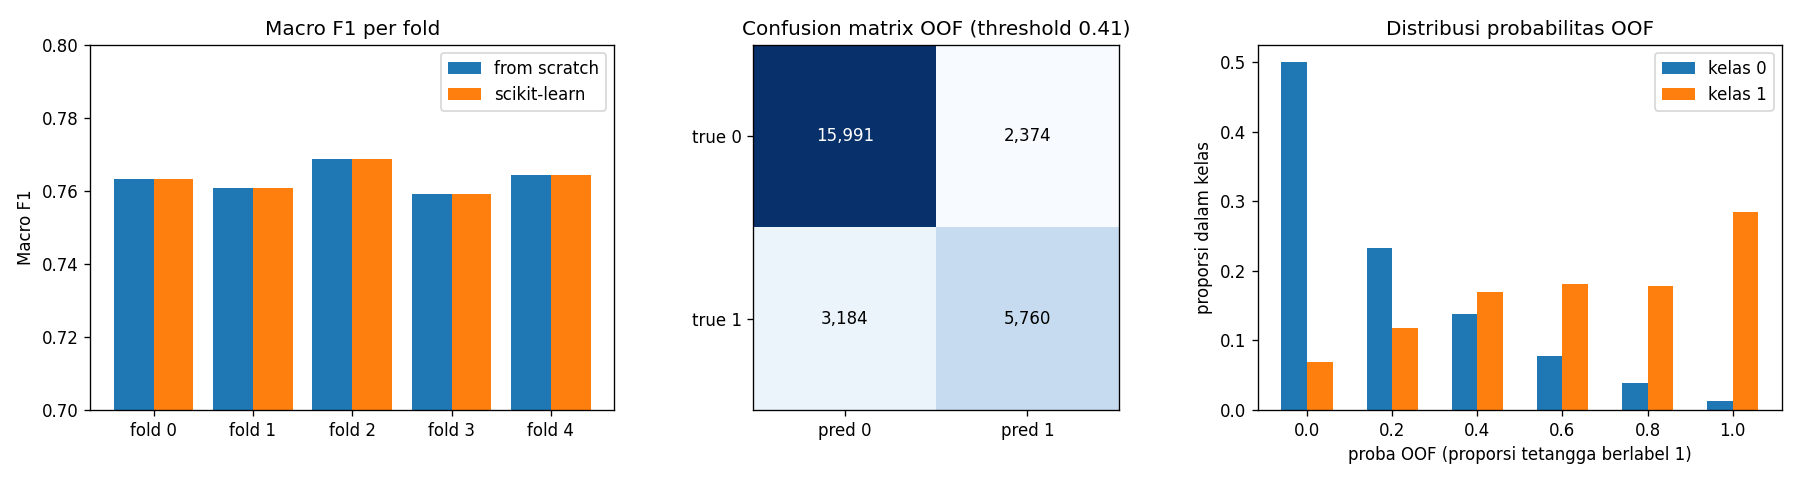
\includegraphics[width=\textwidth]{knn_baseline_comparison.png}
\caption{KNN baseline: Macro F1 per fold, confusion matrix OOF, dan distribusi probabilitas OOF}
\label{fig:knn_baseline}
\end{figure}

\begin{figure}[H]
\centering
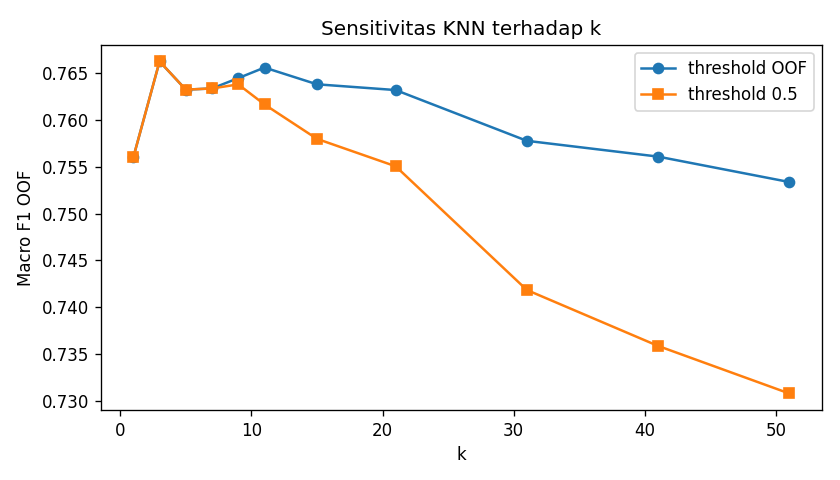
\includegraphics[width=0.65\textwidth]{knn_baseline_k_sweep.png}
\caption{Sensitivitas $k$ pada KNN baseline}
\label{fig:knn_ksweep}
\end{figure}

\subsection{Perkembangan KNN}

\begin{table}[H]
\centering
\caption{Perkembangan konfigurasi KNN sampai model final}
\label{tab:knn_progres}
\begin{tabularx}{\textwidth}{>{\raggedright\arraybackslash}p{4.6cm}X rr}
\toprule
Notebook & Perubahan & OOF & Public \\
\midrule
\texttt{knn\_baseline} & Euclidean, $k=5$, seragam, 39 kolom & 0,7632 & -- \\
\texttt{knn\_forward\_selection} & Forward selection 7 fitur, Manhattan, $k=15$, vote terbobot jarak & 0,8373 & 0,84872 \\
\texttt{knn\_selection\_distance} & Seleksi fitur dengan vote terbobot jarak, 8 fitur, $k=19$ & 0,8411 & 0,85505 \\
\texttt{knn\_feature\_weight} & Bobot fitur hasil coordinate search & 0,8453 & 0,85469 \\
\texttt{knn\_robust\_clip\_minkowski\_weighted} & Dedupe, data error, clipping, robust scaler, $p=1{,}5$, bobot $1/d^2$, $k=19$, 15 fitur & 0,8481 & 0,864 \\
\texttt{knn\_robust\_clip\_minkowski\_weighted\_twin} & + vote booking kembar (toleransi lead 5 hari, tanggal 5 hari) & 0,8520\textsuperscript{b} & 0,87119 \\
model final (\texttt{src/main.ipynb}) & Toleransi lead 10 hari, tanggal 2 hari, harga 6\%, $\alpha=0{,}8$, threshold 0,4845 & 0,8531\textsuperscript{b} & \todo{} \\
\bottomrule
\end{tabularx}

\raggedright\footnotesize \textsuperscript{b} Rata-rata OOF pada tiga seed fold (4, 5, 42) dengan threshold tetap, karena perbedaan antarkonfigurasi kembar sangat kecil.
\end{table}

\subsection{Model final: KNN dengan vote booking kembar}

\begin{table}[H]
\centering
\caption{KNN final: holdout, OOF, dan perbandingan dengan scikit-learn}
\label{tab:knn_final}
\begin{tabular}{lr}
\toprule
Metrik & Nilai \\
\midrule
Macro F1 holdout, KNN + kembar & 0,8592 \\
Macro F1 holdout, KNN saja & 0,8539 \\
Macro F1 OOF 5-fold, KNN + kembar (threshold 0,4845) & 0,8529 \\
Macro F1 OOF 5-fold, KNN saja & 0,8476 \\
Confusion matrix OOF [TN, FP; FN, TP] & [16.728, 1.637; 1.877, 7.067] \\
F1 kelas 0 / kelas 1 (OOF) & 0,9049 / 0,8009 \\
Macro F1 holdout KNN scikit-learn vs from scratch & 0,8539 vs 0,8539 \\
Selisih probabilitas maksimum terhadap scikit-learn & sekitar $10^{-7}$ \\
\bottomrule
\end{tabular}
\end{table}

\begin{figure}[H]
\centering
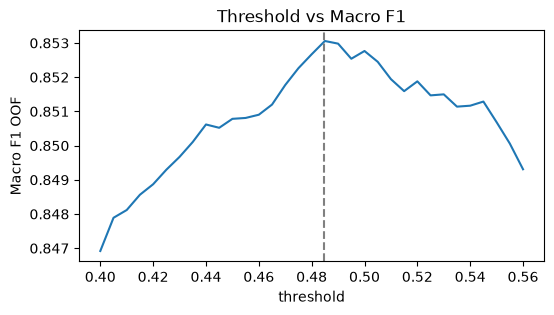
\includegraphics[width=0.6\textwidth]{knn_threshold.png}
\caption{Macro F1 OOF KNN final terhadap threshold}
\label{fig:knn_threshold}
\end{figure}

Setiap pilihan preprocessing dan parameter kembar diuji ulang dengan mengganti satu pilihan dan mempertahankan yang lain (Tabel~\ref{tab:knn_audit}). Semua angka adalah rata-rata OOF pada tiga seed fold dengan threshold 0,48.

\begin{table}[H]
\centering
\caption{Uji pilihan preprocessing dan vote kembar (rata-rata OOF 3 seed fold)}
\label{tab:knn_audit}
\small
\begin{tabular}{llr}
\toprule
Bagian & Varian & OOF \\
\midrule
Dasar & robust, clip 0,5\%, median, $1/d^2$, kembar 10/2/5\% & 0,8528 \\
\midrule
\multirow{3}{*}{Scaler} & z-score & 0,8498 \\
 & rank & 0,8463 \\
 & min-max & 0,8444 \\
\midrule
\multirow{3}{*}{Missing} & imputasi sebelum fitur turunan & 0,8524 \\
 & kategori kosong menjadi one-hot nol & 0,8513 \\
 & jarak mengabaikan kolom kosong & 0,8465 \\
\midrule
\multirow{2}{*}{Bobot vote} & $1/d$ & 0,8516 \\
 & Gaussian & 0,8473 \\
\midrule
\multirow{3}{*}{Clipping} & persentil 1\% & 0,8525 \\
 & IQR $\times3$ & 0,8529 \\
 & tanpa clipping & 0,8529 \\
\midrule
\multirow{3}{*}{Toleransi kembar} & lead 5, tanggal 5 hari & 0,8520 \\
 & lead 12, tanggal 2 hari & 0,8526 \\
 & harga 0\% / 2\% / 10\% & 0,8497 / 0,8521 / 0,8523 \\
\midrule
\multirow{4}{*}{Bobot kembar} & $\alpha$ = 0,5 / 0,6 & 0,8516 / 0,8525 \\
 & $\alpha$ = 0,9 / 1,0 & 0,8524 / 0,8506 \\
 & minimal 1 kembar & 0,8511 \\
 & minimal 3 kembar & 0,8527 \\
\midrule
Final & harga 6\%, $\alpha=0{,}8$, threshold 0,4845 & \textbf{0,8531} \\
\bottomrule
\end{tabular}
\end{table}

\subsection{Analisis KNN}
\begin{enumerate}
  \item \textbf{Kebenaran implementasi.} Pada baseline, probabilitas OOF from scratch identik dengan scikit-learn di seluruh 27.309 baris. Pada konfigurasi final, selisih probabilitas maksimum hanya sekitar $10^{-7}$ (presisi float32) dan Macro F1 holdout sama persis.
  \item \textbf{Representasi fitur paling menentukan.} KNN yang sama naik dari 0,7632 ke 0,8481 hanya dengan seleksi fitur, bobot fitur, robust scaler, clipping, dan jarak Minkowski $p=1{,}5$. Fitur yang tidak relevan ikut menentukan jarak dengan bobot yang sama, sehingga membuangnya memberi kenaikan terbesar.
  \item \textbf{Robust scaler dan jarak $p=1{,}5$.} Z-score, min-max, dan rank terpengaruh ekor panjang lead time dan harga. Jarak $p=1{,}5$ berada di antara Manhattan dan Euclidean sehingga satu kolom dengan selisih besar tidak terlalu mendominasi.
  \item \textbf{Vote booking kembar.} Pemesanan kembar hampir selalu berlabel sama (93,2\%), tetapi lead time-nya berbeda beberapa hari karena noise. KNN biasa dapat melewatkan kembar ini, sedangkan vote kembar memakainya secara langsung. Holdout naik dari 0,8539 ke 0,8592 dan OOF dari 0,8476 ke 0,8529. Toleransi lead time 10 hari lebih baik daripada 5 hari, sesuai temuan bahwa noise ada pada lead time.
  \item \textbf{Area yang datar.} Variasi parameter kembar di sekitar konfigurasi final hanya mengubah OOF sekitar $\pm0{,}001$. Konfigurasi berada di area yang stabil, bukan puncak sempit.
\end{enumerate}

\section{Hasil Decision Tree}

\begin{table}[H]
\centering
\caption{Perkembangan Decision Tree (OOF seed 42 dan rata-rata seed 1 sampai 5)}
\label{tab:dtl_progres}
\begin{tabularx}{\textwidth}{>{\raggedright\arraybackslash}p{3.4cm}X rrrrr}
\toprule
Notebook & Perubahan & OOF & Std & Seed 1--5 & Leaf & Public \\
\midrule
\texttt{dtl\_baseline\_no\_fe} & CART gini, depth 12, leaf 10 & 0,8271 & 0,0031 & 0,8249 & 470 & -- \\
\texttt{dtl\_baseline\_fe} & + 7 fitur turunan & 0,8291 & 0,0076 & 0,8293 & 459 & 0,83740 \\
\texttt{dtl\_gini\_mingain} & min gain $2\times10^{-4}$, depth 30, leaf 5 & 0,8310 & 0,0054 & 0,8322 & 140 & 0,84473 \\
\texttt{dtl\_entropy\_mingain} & entropy, min gain $4{,}5\times10^{-4}$, leaf 3 & 0,8332 & 0,0045 & 0,8315 & 150 & -- \\
\texttt{dtl\_gain\_ratio} & gain ratio (C4.5), min gain $2\times10^{-4}$, leaf 5 & \textbf{0,8343} & \textbf{0,0028} & \textbf{0,8350} & 253 & \textbf{0,84679} \\
\bottomrule
\end{tabularx}
\end{table}

\begin{figure}[H]
\centering
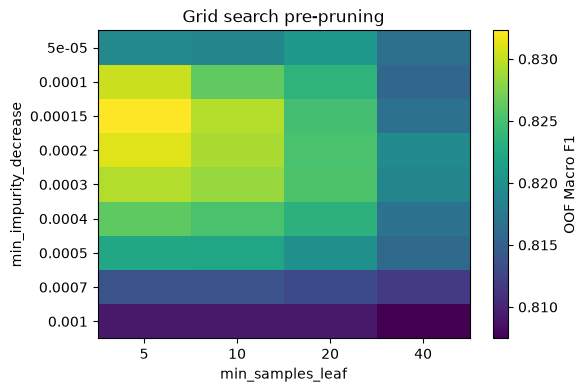
\includegraphics[width=0.48\textwidth]{dtl_grid_gini.png}\hfill
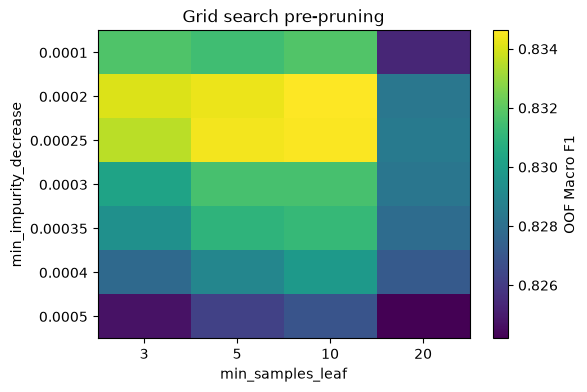
\includegraphics[width=0.48\textwidth]{dtl_grid_gain_ratio.png}
\caption{Grid search pre-pruning (Macro F1 OOF): gini (kiri) dan gain ratio (kanan)}
\label{fig:dtl_grid}
\end{figure}

\begin{table}[H]
\centering
\caption{Decision Tree: from scratch vs scikit-learn pada holdout}
\label{tab:dtl_sklearn}
\begin{tabular}{lrr}
\toprule
Model & Jumlah leaf & Macro F1 holdout \\
\midrule
DTL from scratch (gain ratio) & 273 & \textbf{0,8372} \\
scikit-learn, parameter sama (entropy) & 480 & 0,8297 \\
scikit-learn ID3 (entropy, tanpa batas) & 2.513 & 0,8120 \\
scikit-learn C4.5 (entropy + \texttt{ccp\_alpha} $3\times10^{-4}$) & 343 & 0,8366 \\
scikit-learn CART (gini, tanpa batas) & 2.661 & 0,8063 \\
\bottomrule
\end{tabular}
\end{table}

\begin{table}[H]
\centering
\caption{Cost-complexity pruning pada pohon gain ratio (OOF seed 42)}
\label{tab:dtl_ccp}
\begin{tabular}{rrr}
\toprule
\texttt{ccp\_alpha} & Rata-rata leaf & Macro F1 OOF \\
\midrule
0 sampai $2\times10^{-4}$ & 278 & 0,8343 \\
$3\times10^{-4}$ & 218 & \textbf{0,8348} \\
$5\times10^{-4}$ & 145 & 0,8338 \\
$8\times10^{-4}$ & 96 & 0,8267 \\
$1{,}2\times10^{-3}$ & 61 & 0,8140 \\
\bottomrule
\end{tabular}
\end{table}

\begin{figure}[H]
\centering
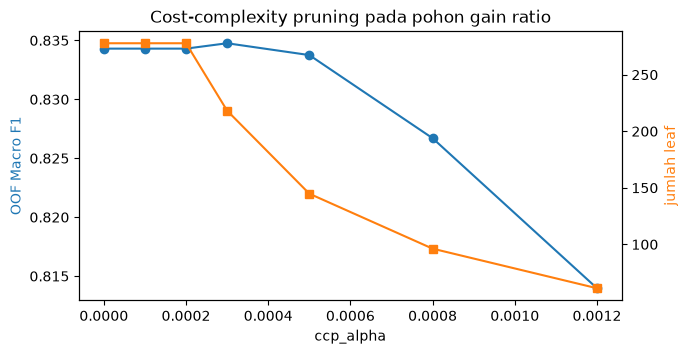
\includegraphics[width=0.65\textwidth]{dtl_ccp.png}
\caption{Cost-complexity pruning: \texttt{ccp\_alpha} terhadap skor dan ukuran pohon}
\label{fig:dtl_ccp}
\end{figure}

\begin{figure}[H]
\centering
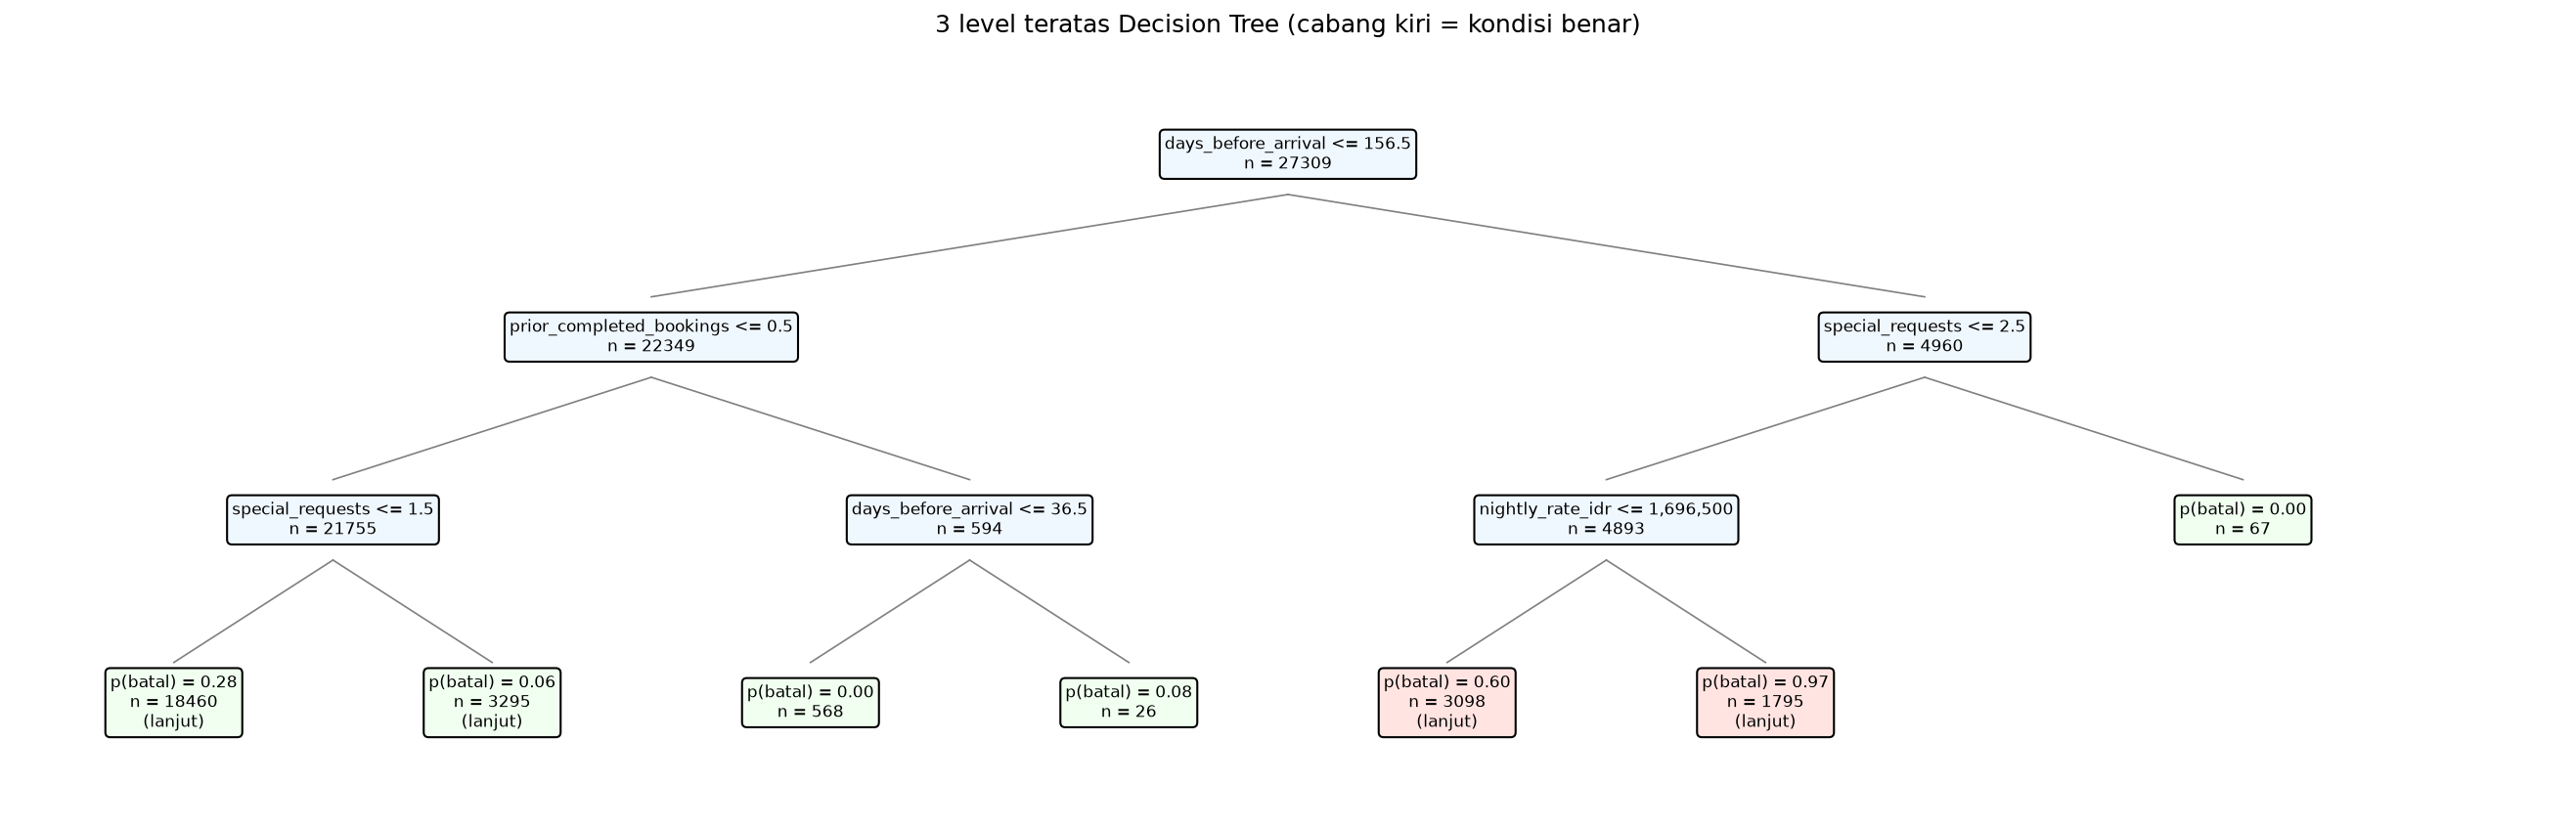
\includegraphics[width=\textwidth]{dtl_tree_top3.png}
\caption{Tiga level teratas pohon DTL final (\texttt{plot\_tree} dengan \texttt{top\_n=3})}
\label{fig:dtl_tree}
\end{figure}

\paragraph{Analisis Decision Tree.}
\begin{enumerate}
  \item \textbf{Pruning paling menentukan.} Pohon tanpa batas (scikit-learn ID3 dan CART, lebih dari 2.500 leaf) paling rendah karena overfit. Pre-pruning dengan minimum gain memangkas pohon dari 459 menjadi 140 leaf sekaligus menaikkan OOF di 5 dari 5 seed fold.
  \item \textbf{Gain ratio paling stabil.} Gain ratio mendapat OOF tertinggi, simpangan baku antar-fold terkecil (0,0028), dan public tertinggi (0,84679). Information gain cenderung memilih split yang memecah data sangat tidak seimbang, sedangkan gain ratio menormalkannya dengan split information.
  \item \textbf{Kenaikan harus dicek di seed lain.} Entropy dengan min gain $4{,}5\times10^{-4}$ naik di seed 42 (0,8332) tetapi turun rata-rata di seed 1 sampai 5 (0,8315 vs 0,8322). Kenaikan di satu pembagian fold dapat hanya kebetulan.
  \item \textbf{Categorical dan missing langsung di pohon.} DTL from scratch membaca 19.933 nilai kosong dan 3 kolom kategorikal tanpa imputasi maupun one-hot, dan unggul atas scikit-learn dengan parameter yang sama yang membutuhkan one-hot dan imputasi (0,8372 vs 0,8297).
  \item \textbf{Cost-complexity pruning.} $\alpha$ sampai $2\times10^{-4}$ tidak memangkas apa pun karena minimum gain $2\times10^{-4}$ sudah mencegah split sekecil itu. $\alpha=3\times10^{-4}$ memangkas 22\% leaf dan sedikit menaikkan OOF, sedangkan $\alpha$ yang terlalu besar menyebabkan underfit. Versi dengan pruning ini mendapat public 0,84604, sedikit di bawah versi tanpa pruning, sehingga model final tetap tanpa pruning.
  \item \textbf{Struktur pohon.} Split pertama adalah lead time 156,5 hari. Pemesanan jauh hari dengan special requests paling banyak 2 dan harga di atas sekitar Rp1,7 juta hampir pasti batal (97\%), sedangkan tamu lama dengan lead time di bawah 37 hari tidak ada yang batal.
\end{enumerate}

\section{Hasil Logistic Regression}

\begin{table}[H]
\centering
\caption{Tahapan tuning Logistic Regression (OOF seed 42)}
\label{tab:lr_tahap}
\begin{tabularx}{\textwidth}{>{\raggedright\arraybackslash}p{3cm}X rr}
\toprule
Tahap & Perubahan & OOF & Public \\
\midrule
baseline & Data tanpa feature engineering, L2 & 0,7595 & -- \\
threshold & + tuning threshold (0,45) & 0,7671 & -- \\
\texttt{lr\_fe} & Bin kuantil, one-hot, interaksi 14 fitur, L2 & 0,8231 & 0,82860 \\
\texttt{lr\_target\_bins} & Bin berbasis target (16 bin), L2 dengan $C=0{,}01$ & 0,8276 & 0,83176 \\
\texttt{lr\_l1\_onehot} & One-hot jumlah tamu, L1 & 0,8297 & 0,83480 \\
\texttt{lr\_cross\_bins} & + sel dua dimensi lead time $\times$ waktu kedatangan, 2.814 kolom & \textbf{0,8344} & \textbf{0,83542} \\
\bottomrule
\end{tabularx}
\end{table}

Dengan preprocessing bersama (28 kolom), Logistic Regression hanya mendapat 0,7644 (\texttt{lr\_main\_prep}). Dengan ekspansi fitur khusus model linear di atas preprocessing bersama (\texttt{lr\_main\_expand}), skornya naik ke 0,8225, dan grid regularisasi menghasilkan L1, L2, dan Elastic Net yang hampir setara (0,8194 sampai 0,8225).

\begin{table}[H]
\centering
\caption{Logistic Regression: from scratch vs scikit-learn (\texttt{lr\_cross\_bins}, holdout)}
\label{tab:lr_sklearn}
\begin{tabular}{lrrrr}
\toprule
Model & Iterasi & Bobot tidak nol & Log-loss & Macro F1 \\
\midrule
From scratch L2 (FISTA) & 1.337 & 2.814 & 0,36342 & 0,8273 \\
From scratch L1 (FISTA) & 432 & 1.234 & 0,33452 & 0,8330 \\
scikit-learn L2 (lbfgs) & 532 & 2.814 & 0,36329 & 0,8272 \\
\bottomrule
\end{tabular}
\end{table}

\begin{figure}[H]
\centering
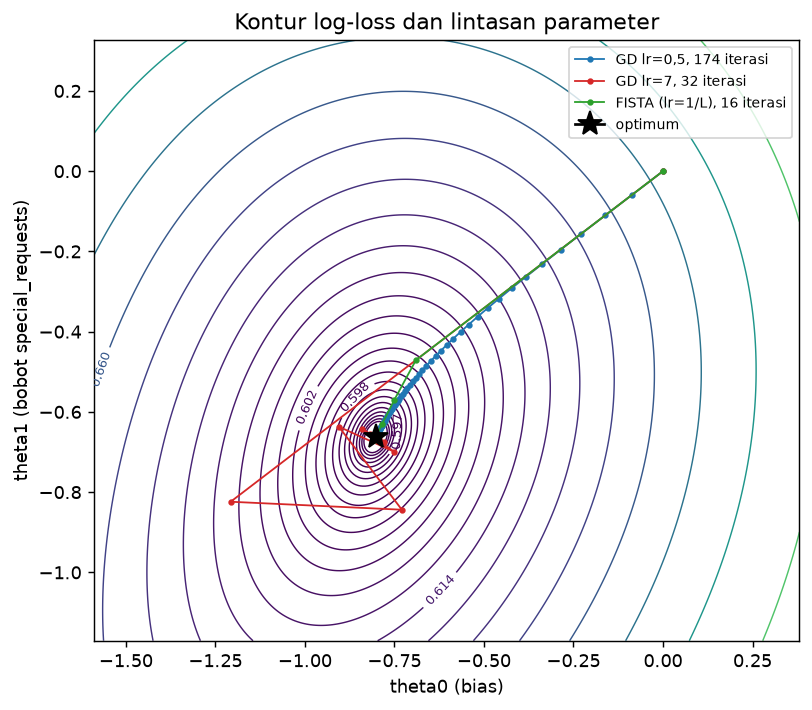
\includegraphics[width=0.75\textwidth]{lr_cross_bins_contour.png}
\caption{Kontur log-loss dan lintasan parameter $(\theta_0,\theta_1)$ selama training (cuplikan video bonus)}
\label{fig:lr_contour}
\end{figure}

\paragraph{Analisis Logistic Regression.}
\begin{enumerate}
  \item \textbf{Kebenaran implementasi.} Objektif L2 from scratch (0,258208) hampir sama dengan scikit-learn (0,258200), dengan Macro F1 holdout 0,8273 vs 0,8272.
  \item \textbf{Model linear butuh representasi tidak linear.} Hubungan lead time dengan pembatalan tidak linear, sehingga satu bobot per fitur tidak cukup. Binning, interaksi, dan sel dua dimensi menaikkan OOF dari 0,7671 ke 0,8344.
  \item \textbf{L1 sebagai seleksi fitur.} Pada 2.814 kolom, L1 hanya mempertahankan 1.234 bobot tidak nol dan memberi log-loss lebih rendah.
  \item \textbf{FISTA lebih cepat.} Pada contoh dua parameter, gradient descent butuh 174 iterasi (learning rate 0,5) atau 32 iterasi (learning rate 7), sedangkan FISTA hanya 16 iterasi untuk mencapai loss yang sama (0,59674).
\end{enumerate}

\section{Hasil Support Vector Machine}
\begingroup
\setlength{\emergencystretch}{3em}
\subsection{Perkembangan eksperimen dan submission}
Eksperimen SVM dimulai dari kernel linear, dilanjutkan dengan tuning linear, Gaussian, polynomial, lalu pipeline final (Tabel~\ref{tab:svm_history}). Empat hasil awal dicatat dengan solver SMO dan seed fold 42. Notebook saat ini sudah memakai dekomposisi SLSQP, tetapi keempat eksperimen tersebut belum seluruhnya dijalankan ulang. SVM final diuji dengan seed 5 dan preprocessing template. Perbedaan ini perlu diperhatikan saat membandingkan kenaikan skor karena pengaruh tiap perubahan belum diuji secara terpisah.
\begin{table}[H]
\centering
\caption{Perkembangan SVM (tanda -- berarti skor public belum teridentifikasi)}
\label{tab:svm_history}
\begin{tabular}{lrrrr}
\toprule
Eksperimen & Threshold & Macro F1 OOF & Std fold & Public \\
\midrule
Linear baseline, $C=0{,}01$ & 0,45 & 0,7656 & 0,0050 & 0,77484 \\
Linear tuning, $C=0{,}1$ & 0,44 & 0,7659 & 0,0053 & -- \\
Gaussian historis, $C=1$ & 0,43 & 0,7907 & 0,0036 & -- \\
Polynomial, $C=1$, $d=3$ & 0,40 & 0,7943 & 0,0034 & 0,81212 \\
\textbf{SVM final}, Gaussian & 0,25 & \textbf{0,83243} & 0,00526 & \textbf{0,85189} \\
\bottomrule
\end{tabular}
\end{table}
Pada eksperimen awal, Gaussian dan polynomial mengungguli linear sekitar 0,025 sampai 0,029 Macro F1. Batas keputusan nonlinear memberi hasil lebih baik pada representasi fitur tersebut. SVM final kemudian naik 0,03809 OOF dan 0,03977 public dibandingkan polynomial awal. Kenaikan ini terjadi setelah preprocessing, konfigurasi, dan seed diubah, sehingga kontribusi masing-masing perubahan masih perlu diperiksa melalui ablation.

Submission SVM final adalah \texttt{output/submissions/submission\_svm\_final.csv}, diterima Kaggle dengan ID \texttt{58803590}, status \texttt{COMPLETE}, dan public score \textbf{0,85189}. Skor private belum tersedia.
Skor public berasal dari sebagian data test di Kaggle, sedangkan OOF dihitung dari train. Selisih keduanya tidak dapat dibandingkan langsung karena datanya berbeda. SVM menjadi submission eksperimen, sementara model final kelompok tetap KNN.

\subsection{Perbandingan dengan scikit-learn dan analisis kesalahan}
\begin{table}[H]
\centering
\caption{Perbandingan penuh SVM final, $C=0{,}3$, $\gamma=1$}
\label{tab:svm}
\begin{tabular}{lrrr}
\toprule
Model & Threshold & Macro F1 OOF & Std fold \\
\midrule
From scratch & 0,25 & 0,832426 & 0,005263 \\
scikit-learn SVC terkalibrasi & 0,27 & 0,832468 & 0,004459 \\
\bottomrule
\end{tabular}
\end{table}
Macro F1 kedua model hanya berselisih 0,000042 pada data, preprocessing, dan fold luar yang sama. Threshold terpilih berbeda karena solver dan cara kalibrasinya dapat menghasilkan probabilitas berbeda. Skor lima fold from scratch berturut-turut adalah 0,82747, 0,82894, 0,83542, 0,82889, dan 0,84139. Semua model fold memenuhi pemeriksaan konvergensi tanpa peringatan. Nilai std dihitung sebagai standar deviasi populasi dari lima skor tersebut dan tidak menyatakan interval kepercayaan.

\begin{figure}[H]
\centering
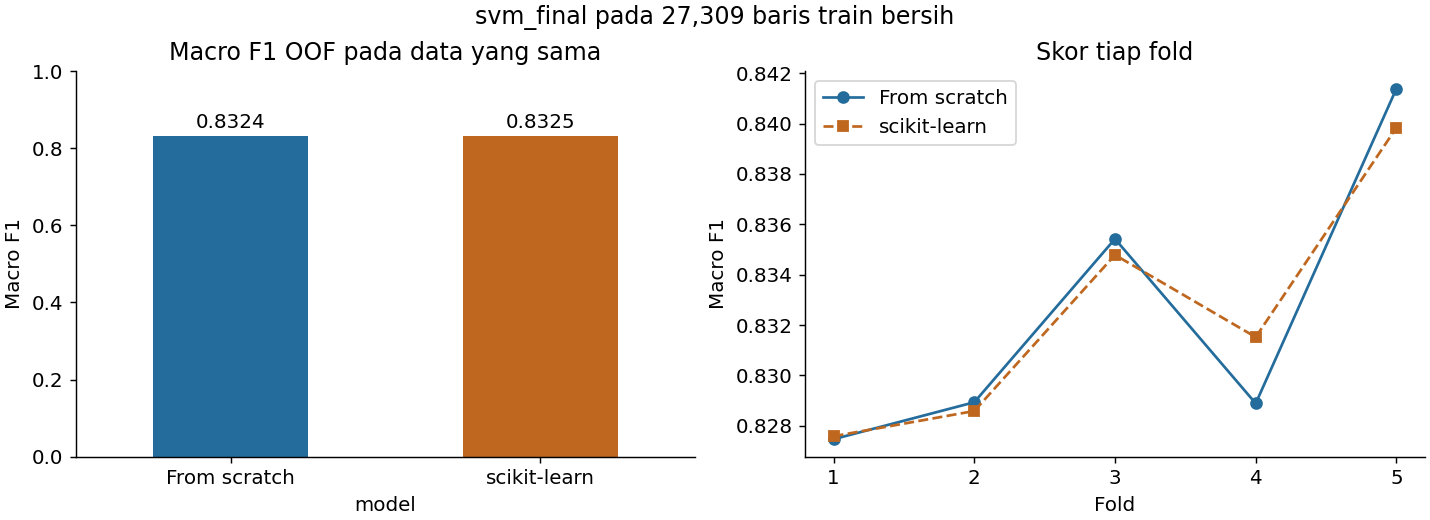
\includegraphics[width=0.78\textwidth]{svm_final_comparison.png}
\caption{Macro F1 OOF dan skor tiap fold SVM final dibandingkan scikit-learn}
\label{fig:svm_comparison}
\end{figure}

Confusion matrix OOF from scratch adalah $\bigl[\begin{smallmatrix}16186&2179\\1886&7058\end{smallmatrix}\bigr]$, dengan urutan baris kelas aktual 0 dan 1 serta kolom kelas prediksi 0 dan 1. Terdapat 2.179 FP dan 1.886 FN. Threshold 0,25 dipilih berdasarkan Macro F1 dari probabilitas yang sudah dikalibrasi. Pemilihan ini belum mempertimbangkan biaya $2FP+FN$. Jumlah FP saja juga belum cukup untuk menilai apakah probabilitas terlalu ekstrem atau kalibrasinya buruk. Eksperimen cost-sensitive kelompok dibahas pada bagian tersendiri dengan model yang digunakan di sana.

\begin{figure}[H]
\centering
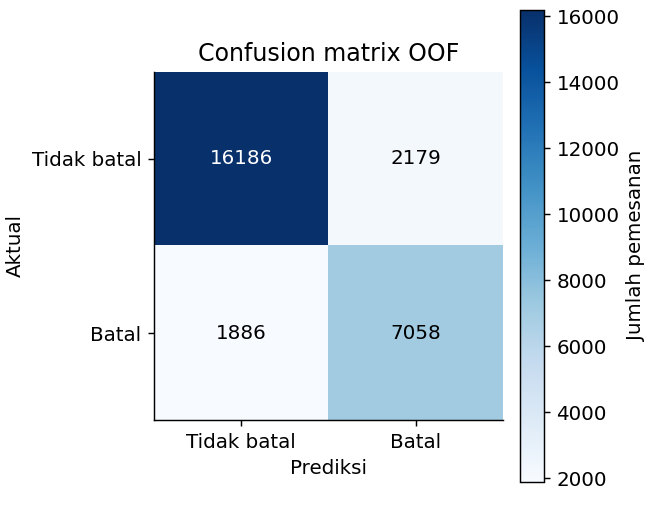
\includegraphics[width=0.61\textwidth]{svm_final_confusion_matrix.png}
\caption{Confusion matrix OOF SVM final dengan threshold 0,25}
\label{fig:svm_confusion}
\end{figure}

\subsection{Bonus bidang pemisah, margin, dan support vector}
Visualisasi ketiga kernel pada Gambar~\ref{fig:svm_boundaries} memakai dua fitur: \texttt{days\_before\_arrival} dan \texttt{nightly\_rate\_idr}. Sebanyak 400 sampel dipilih dengan seed 5, diimputasi median dan distandardisasi berdasarkan sampel visualisasi tersebut. Tiga model dua dimensi dilatih khusus untuk gambar dengan $C=1$, $d=3$, $r=1$, dan \texttt{gamma='scale'} untuk kernel nonlinear. Ketiga model ini dilatih khusus pada dua fitur tersebut. Model submission tetap memakai 28 kolom, dengan konfigurasi dan jumlah support vector yang berbeda.

Garis penuh menunjukkan $f(x)=0$, garis putus-putus menunjukkan $f(x)=\pm1$, dan lingkaran menandai support vector. Warna serta bentuk marker membedakan kelas. Jumlah support vector adalah 226 untuk linear, 207 untuk polynomial, dan 216 untuk Gaussian. Kurva nonlinear mengikuti bentuk yang tidak dapat ditangkap satu garis lurus. Pada soft margin, support vector dapat berada di batas maupun di dalam margin. Untuk kernel nonlinear, jarak antarkontur pada bidang masukan tidak menunjukkan lebar margin Euclidean yang konstan.

\begin{figure}[H]
\centering
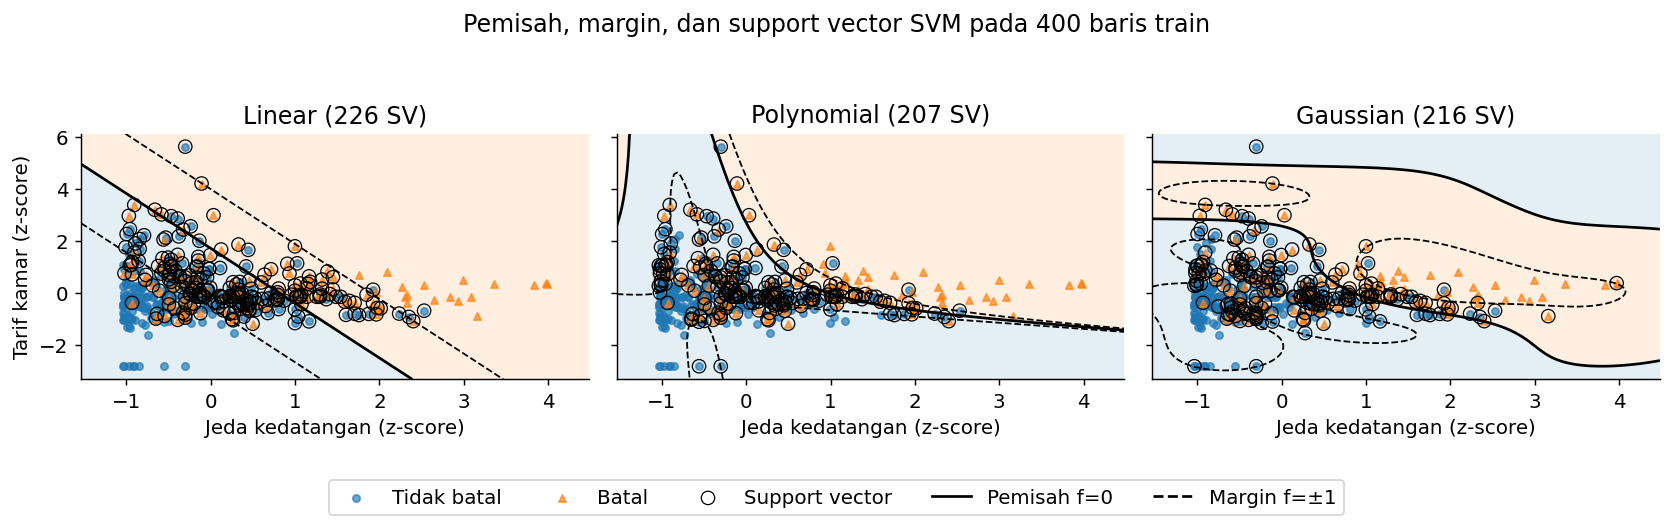
\includegraphics[width=\textwidth]{svm_final_boundaries.png}
\caption{Bidang pemisah, margin, dan support vector pada tiga kernel SVM}
\label{fig:svm_boundaries}
\end{figure}

\subsection{Hasil bonus PSO dan keterbatasan}
\begin{table}[H]
\centering
\caption{PSO pada 800 baris development dan 400 baris holdout}
\label{tab:svm_pso}
\begin{tabular}{lrrrrr}
\toprule
Model & $C$ & $\gamma$ & Threshold & OOF dev & Holdout \\
\midrule
Baseline & 0,30000 & 1,00000 & 0,36 & 0,77046 & 0,80387 \\
PSO terpilih & 0,44287 & 0,49811 & 0,35 & 0,77959 & 0,79404 \\
\bottomrule
\end{tabular}
\end{table}
PSO menyelesaikan 32 evaluasi dalam sekitar 133,7 detik. Skor OOF development naik 0,00913, tetapi skor holdout turun 0,00983. Parameter yang terpilih lebih cocok untuk development dan belum memberi perbaikan pada holdout. Pencarian pada sampel kecil ini masih rentan terhadap bias seleksi. Holdout juga hanya terpisah dalam eksperimen bonus karena pemilihan kernel sebelumnya sudah memakai seluruh train. Dengan satu seed dan ruang pencarian terbatas, hasil PSO belum menjamin konfigurasi terbaik atau peningkatan generalisasi. Karena itu, submission final tetap memakai konfigurasi sebelum PSO.

\begin{figure}[H]
\centering
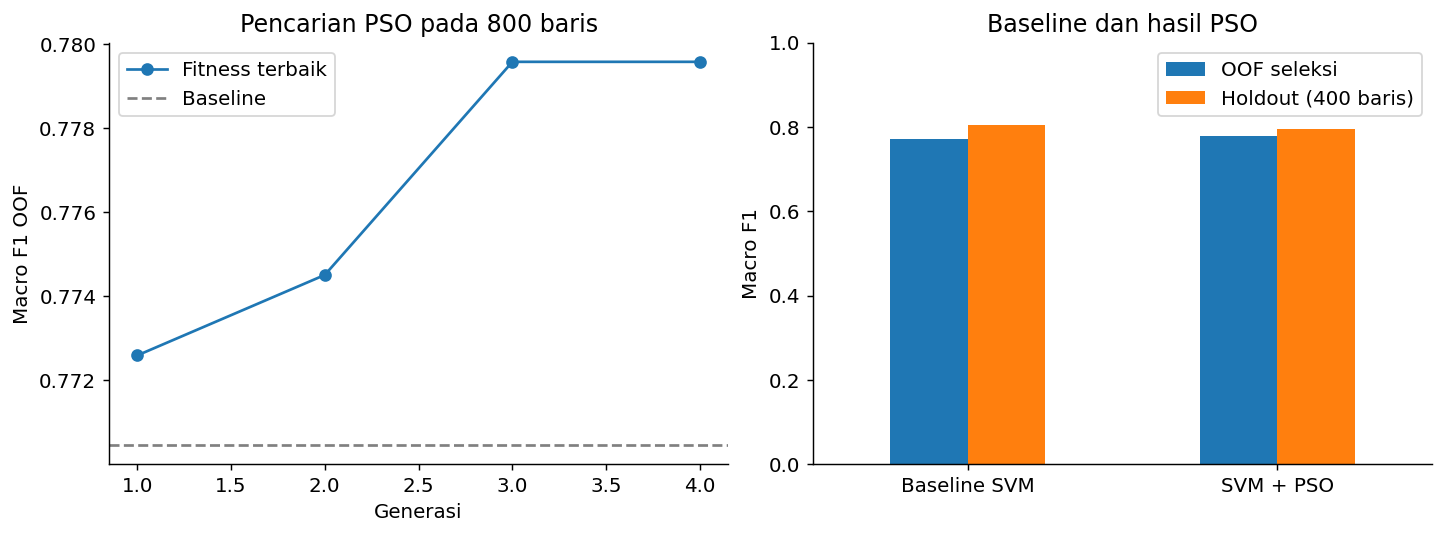
\includegraphics[width=0.95\textwidth]{svm_final_pso.png}
\caption{Perkembangan fitness terbaik PSO serta perbandingan development dan holdout}
\label{fig:svm_pso}
\end{figure}


\endgroup
\section{Hasil Naive Bayes}
\subsection{Perkembangan empat eksperimen}
Tabel~\ref{tab:nb_tahap} membandingkan keempat eksperimen dengan Macro F1 OOF pada protokol tim. Kolom Public memuat skor leaderboard Kaggle untuk baseline 17 fitur, fine-tuning, dan varian kontekstual. Varian dua fitur yang mendahuluinya memakai \texttt{booking\_channel} dan \texttt{special\_requests} dan memperoleh 0,6652 OOF.

\begin{table}[H]
\centering
\caption{Hasil empat eksperimen Naive Bayes pada validasi dan Kaggle}
\label{tab:nb_tahap}
\begin{tabularx}{\textwidth}{p{3.0cm}Xrrrr}
\toprule
Tahap & Perubahan & Threshold & Macro F1 & Std fold & Public \\
\midrule
Baseline & 17 fitur asli, \(\alpha=1\) & 0,42 & 0,73422 & 0,00841 & 0,73697 \\
Fine-tuning & \(\alpha=2\), bobot fitur 2 & 0,49 & 0,73984 & 0,00482 & 0,74192 \\
Smoothing per\newline fitur & \(\alpha=10\) untuk permintaan & 0,49 & 0,73977 & 0,00460 & -- \\
Kontekstual & Bin kontekstual, 9 masukan & 0,43 & \textbf{0,80196} & 0,00729 & \textbf{0,80173} \\
\bottomrule
\end{tabularx}
\end{table}

\begin{figure}[htbp]
\centering
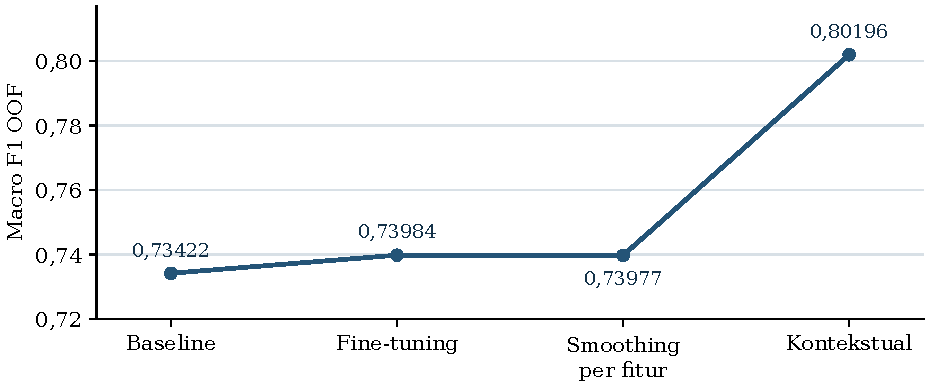
\includegraphics[width=0.84\textwidth]{nb_macro_f1.pdf}
\caption{Perubahan Macro F1 OOF antar-eksperimen pada protokol tim.}
\label{fig:nb_oof}
\end{figure}

Fine-tuning menaikkan Macro F1 sebesar 0,00562 dan memperbaiki empat dari lima fold. Dibanding baseline, false positive turun dari 3.917 ke 3.252, sedangkan false negative naik dari 2.688 ke 3.044. Smoothing per fitur menghasilkan perubahan total \(-0{,}00007\), walaupun tiga fold membaik tipis. Pada konfigurasi ini, smoothing yang lebih kuat untuk satu fitur belum menambah daya prediksi. Perubahan terbesar muncul pada tahap kontekstual, dengan kenaikan 0,06219 terhadap tahap sebelumnya. Karena tahap tersebut sekaligus mengubah diskretisasi, susunan fitur, dan pemilihan parameter, selisihnya mengukur efek gabungan.

\subsection{Validasi bertingkat dan perbandingan dengan scikit-learn}
Konfigurasi ekspor memperoleh OOF seleksi 0,80328 dengan threshold 0,45. Skor ini ikut menentukan konfigurasi yang dipilih. Validasi bertingkat memperoleh 0,79943 pada gabungan prediksi fold luar dan unggul pada lima fold terhadap \texttt{nb\_categorical\_tuned}, pembanding lama yang memakai bin hari rinci, kuantil tarif, dan gabungan kanal dengan rentang hari. Pembanding tersebut menggunakan prosedur validasi bertingkat yang sama dan berbeda dari baseline 17 fitur pada Tabel~\ref{tab:nb_tahap}.

\begin{table}[H]
\centering
\caption{Macro F1 pada fold luar validasi bertingkat kontekstual}
\label{tab:nb_nested}
\begin{tabular}{lrrr}
\toprule
Fold luar & Pembanding lama & Kontekstual & Threshold kontekstual \\
\midrule
1 & 0,75828 & 0,81082 & 0,435 \\
2 & 0,75328 & 0,79016 & 0,450 \\
3 & 0,75488 & 0,79297 & 0,475 \\
4 & 0,75433 & 0,80747 & 0,460 \\
5 & 0,74997 & 0,79571 & 0,420 \\
\midrule
OOF gabungan & 0,75421 & \textbf{0,79943} & -- \\
\bottomrule
\end{tabular}
\end{table}

\begin{table}[H]
\centering
\caption{Kesetaraan from scratch dengan pembanding scikit-learn pada konfigurasi yang sama}
\label{tab:nb}
\begin{tabularx}{\textwidth}{Xrrr}
\toprule
Tahap & From scratch & Pembanding & Selisih peluang maks. \\
\midrule
Baseline & 0,73422 & 0,73422 & \(6{,}00\times 10^{-15}\) \\
Fine-tuning (likelihood berbobot) & 0,73984 & 0,73984 & \(5{,}33\times 10^{-15}\) \\
Smoothing per fitur (likelihood berbobot) & 0,73977 & 0,73977 & \(5{,}44\times 10^{-15}\) \\
Kontekstual (OOF seleksi) & 0,80328 & 0,80328 & \(4{,}66\times 10^{-15}\) \\
\bottomrule
\end{tabularx}
\end{table}

Pada fine-tuning, \texttt{CategoricalNB} standar dengan bobot seragam dan \(\alpha=2\) memperoleh 0,73380. Pembanding berbobot memperoleh 0,73984. Selisih peluang pada Tabel~\ref{tab:nb} setara dengan galat pembulatan. Baris kontekstual memakai OOF seleksi karena verifikasi memakai konfigurasi ekspor dan fold yang sama.

\subsection{Analisis kesalahan, reproduksibilitas, dan bonus}
Prediksi gabungan fold luar kontekstual menghasilkan 15.960 \emph{true negative}, 2.444 \emph{false positive}, 2.400 \emph{false negative}, dan 6.569 \emph{true positive}. F1 kelas tidak batal mencapai 0,86824, sedangkan F1 kelas batal mencapai 0,73062. Pada kelompok \emph{lead time} lebih dari 80 hingga 151 hari, tingkat kesalahan masih 25,7\% dari 5.191 baris. Kelompok 11 hari atau kurang memiliki tingkat kesalahan 9,9\% dari 5.293 baris. Hasil ini menunjukkan bahwa kualitas prediksi berbeda antar-kelompok pemesanan setelah diskretisasi kontekstual.

Hasil run ulang \texttt{nb\_baseline} identik byte demi byte dengan \texttt{submission\_nb\_categorical\_all.csv} di branch \texttt{main}, yang mencatat public score 0,73697. Fine-tuning mencapai 0,74192 pada public leaderboard. Varian kontekstual mencapai 0,80173 dengan 6.844 prediksi dan threshold ekspor 0,45. Skor kontekstual 0,80196 dan 0,79943 berasal dari validasi data latih. KNN dengan vote booking kembar tetap menjadi model submission final kelompok.

Gambar~\ref{fig:nb_graf} menampilkan struktur dari sel bonus notebook kontekstual dengan label ringkas. Simpul \texttt{is\_canceled} memiliki sembilan anak sesuai masukan model. Panah menjelaskan faktorisasi peluang kondisional. Masing-masing simpul dapat berupa satu fitur atau satu kategori gabungan.

\begin{figure}[H]
\centering
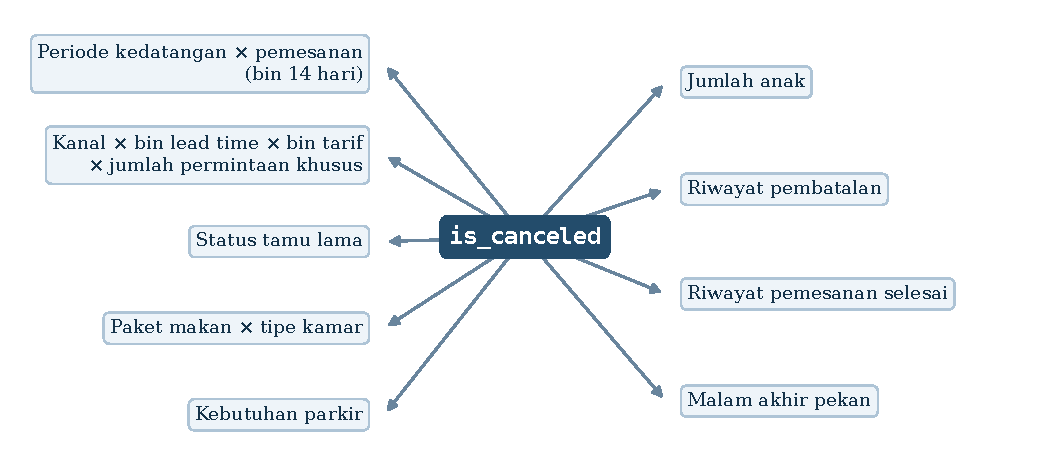
\includegraphics[width=\textwidth]{nb_graf.pdf}
\caption{Graf Bayesian Network untuk konfigurasi Categorical Naive Bayes kontekstual.}
\label{fig:nb_graf}
\end{figure}


\section{Analisis Perbandingan Antar-Model}
\begin{enumerate}
  \item \textbf{Peringkat.} KNN + kembar (0,8529) $>$ KNN (0,8476) $>$ DTL ($\approx$0,834) $\approx$ LR ($\approx$0,834) $>$ SVM final (0,8324) $>$ NB kontekstual (0,8020). Skor public SVM final (0,85189) melebihi DTL dan LR pada tabel ringkasan, sehingga urutan public tidak seluruhnya sama dengan urutan OOF. Skor public NB kontekstual adalah 0,80173. Perbedaan seed dan prosedur seleksi membatasi perbandingan langsung.
  \item \textbf{Representasi fitur lebih menentukan daripada algoritma.} KNN naik dari 0,7632 ke 0,8476 dan LR dari 0,7595 ke 0,8344 hanya dengan mengubah representasi fitur. Decision Tree kuat tanpa banyak rekayasa fitur karena seleksi fitur sudah melekat pada pemilihan split.
  \item \textbf{Memahami cara data dibuat.} Kenaikan terbesar KNN final datang dari analisis noise: pemesanan kembar hampir selalu berlabel sama, dan noise ada pada lead time. Informasi ini dipakai langsung lewat vote kembar.
  \item \textbf{Threshold menggantikan resampling.} Threshold OOF SVM final adalah 0,25, sedangkan banyak eksperimen lain berada sekitar 0,40 sampai 0,53. Karena kelas batal hanya 32,8\%, menurunkan threshold menyeimbangkan recall kelas minoritas dan menaikkan Macro F1 tanpa data sintetis.
  \item \textbf{Kesetaraan dengan pustaka.} Implementasi from scratch setara dengan scikit-learn: KNN dan Naive Bayes identik secara numerik, LR berselisih 0,0001, dan DTL dengan cost-complexity pruning menghasilkan pohon yang sama persis dengan scikit-learn pada parameter yang sama.
\end{enumerate}

\section{Cost-sensitive Classification}
False Positive (diprediksi batal, ternyata datang) lebih mahal karena penginapan dapat overbooked. Diasumsikan biaya FP dua kali FN, sehingga total biaya adalah $2\,FP + FN$. Dengan probabilitas yang terkalibrasi, keputusan dengan biaya harapan minimum adalah memprediksi batal jika $\hat{p}\,C_{FN} > (1-\hat{p})\,C_{FP}$, yaitu $\hat{p} > C_{FP}/(C_{FP}+C_{FN}) = 2/3$ \cite{ref:elkan}. Threshold juga dicari langsung dari prediksi OOF model final.

\begin{table}[H]
\centering
\caption{Pengaruh threshold pada biaya (OOF KNN + kembar)}
\label{tab:cost}
\begin{tabular}{lrrrrrr}
\toprule
Threshold & Nilai & FP & FN & Biaya & Macro F1 & Prediksi batal \\
\midrule
Macro F1 maksimum & 0,4845 & 1.637 & 1.877 & 5.151 & 0,8529 & 31,9\% \\
Teori $2/3$ & 0,6667 & 764 & 2.931 & 4.459 & 0,8350 & 24,8\% \\
Biaya minimum (OOF) & 0,74 & 494 & 3.423 & \textbf{4.411} & 0,8197 & 22,0\% \\
\bottomrule
\end{tabular}
\end{table}

\begin{figure}[H]
\centering
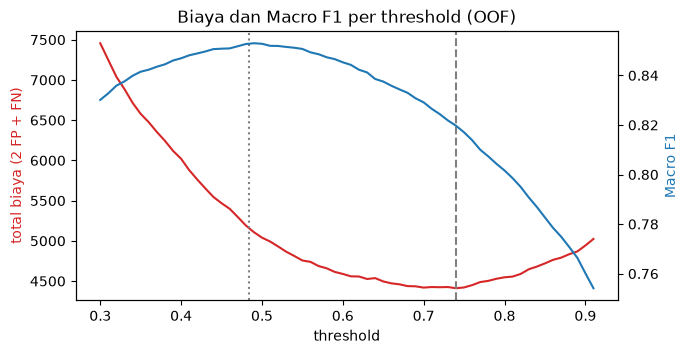
\includegraphics[width=0.65\textwidth]{cost_sensitive.png}
\caption{Total biaya dan Macro F1 terhadap threshold}
\label{fig:cost}
\end{figure}

Dengan biaya FP dua kali FN, threshold dinaikkan dari 0,4845 ke sekitar 0,67 sampai 0,74, dan biaya turun 14\%. FP turun dari 1.637 ke 494, tetapi FN naik dari 1.877 ke 3.423 dan Macro F1 turun ke 0,8197. Model dan preprocessing tidak berubah, yang berubah hanya threshold keputusan. Threshold empiris (0,74) dekat dengan teori (0,67), menandakan probabilitas model cukup terkalibrasi. Untuk kompetisi tetap dipakai threshold Macro F1 karena metrik Kaggle adalah Macro F1.

\section{Ringkasan Bonus}
\begin{table}[H]
\centering
\caption{Bonus yang dikerjakan}
\label{tab:bonus}
\begin{tabularx}{\textwidth}{>{\raggedright\arraybackslash}p{4.2cm}X}
\toprule
Bonus & Keterangan \\
\midrule
Kaggle & Peringkat 1 public leaderboard dengan KNN from scratch, reproducible melalui \texttt{src/main.ipynb} \\
DTL: gambar percabangan & \texttt{plot\_tree(model, top\_n)}, Gambar~\ref{fig:dtl_tree}, berkas \texttt{output/figures/dtl\_tree\_top3.png} \\
LR: video kontur log-loss & \texttt{output/figures/lr\_*\_contour.mp4}, Gambar~\ref{fig:lr_contour} \\
SVM: gambar bidang pemisah & Linear, polynomial, dan Gaussian, termasuk margin serta support vector pada Gambar~\ref{fig:svm_boundaries}, dengan kode pada \texttt{svm\_final.ipynb} \\
Naive Bayes: graf fitur & Graf untuk sembilan masukan kategori terpilih, Gambar~\ref{fig:nb_graf} \\
Algoritma optimasi DTL & Cost-complexity pruning \cite{ref:breiman}, Tabel~\ref{tab:dtl_ccp} \\
Algoritma optimasi LR & FISTA dengan adaptive restart \cite{ref:fista}, Kode~\ref{lst:fista} \\
Algoritma optimasi SVM & PSO untuk $C$ dan $\gamma$, Kode~\ref{lst:svm_pso}, dan Tabel~\ref{tab:svm_pso}. Fitness naik tetapi holdout turun \cite{ref:pso,ref:pso_shi} \\
Algoritma optimasi NB & Diskretisasi MDL, penggabungan kategori, dan seleksi wrapper \cite{ref:fayyad_nb,ref:pazzani_nb,ref:kohavi_nb}, Tabel~\ref{tab:nb_nested} \\
Cost-sensitive classification & Tabel~\ref{tab:cost} \\
\bottomrule
\end{tabularx}
\end{table}

\chapter{Kesimpulan dan Saran}

\section{Kesimpulan}
\begin{enumerate}
  \item KNN, Decision Tree (C4.5 dengan dukungan data numerik, kategorikal, dan missing value), Logistic Regression (L1, L2, dan Elastic Net), SVM (kernel linear, polynomial, dan Gaussian), serta Categorical Naive Bayes berhasil diimplementasikan from scratch. Hasilnya setara dengan scikit-learn pada data dan preprocessing yang sama.
  \item Model terbaik adalah KNN from scratch dengan preprocessing bersama dan vote booking kembar, dengan Macro F1 OOF 0,8529 dan holdout 0,8592. Model ini mencapai peringkat 1 public leaderboard dan direproduksi secara identik oleh \texttt{src/main.ipynb}.
  \item Decision Tree terbaik memakai gain ratio (C4.5) dengan pre-pruning minimum gain (OOF 0,8343, public 0,84679). Cost-complexity pruning dapat memangkas pohon sekitar 22\% tanpa menurunkan skor.
  \item Varian kontekstual mencapai Macro F1 OOF 0,80196 pada protokol tim dan 0,79943 pada validasi bertingkat. Skor public Kaggle varian ini adalah 0,80173. Pada preprocessing tetap, fine-tuning menghasilkan kenaikan kecil dan smoothing per fitur menghasilkan skor yang hampir sama. Pada data ini, perubahan representasi kategori memberi kenaikan yang lebih besar. Uji berikutnya dapat mengukur kontribusi diskretisasi kontekstual dan penggabungan kategori satu per satu pada fold luar yang sama.

  \item Pada dataset ini, representasi fitur dan pemahaman cara data dibuat lebih menentukan daripada pilihan algoritma. Analisis noise pada lead time menghasilkan vote booking kembar, yang memberi kenaikan terbesar pada model final.
  \item Pemilihan threshold dari prediksi OOF efektif menangani ketidakseimbangan kelas 2:1 tanpa resampling. Jika biaya FP dua kali FN, threshold optimal naik ke sekitar 0,67 sampai 0,74 dan biaya turun 14\%.
  \item Setiap perubahan konfigurasi perlu dicek pada beberapa seed fold. Beberapa kenaikan yang terlihat pada satu pembagian fold ternyata tidak konsisten pada seed lain.
\end{enumerate}

\section{Saran}
\begin{enumerate}
  \item Menerapkan seleksi dan pembobotan fitur yang terbukti membantu KNN pada SVM, karena SVM masih memakai seluruh kolom tanpa seleksi.
  \item Memakai ide booking kembar pada model lain, misalnya sebagai fitur tambahan untuk Decision Tree atau Logistic Regression.
  \item Memeriksa stabilitas bin kontekstual pada pembagian data lain, terutama pada kanal dengan sedikit sampel.
  \item Mempercepat KNN from scratch untuk data lebih besar dengan struktur indeks (misalnya KD-tree) atau perhitungan jarak di GPU.
\end{enumerate}

\chapter*{Pembagian Tugas}
\addcontentsline{toc}{chapter}{Pembagian Tugas}

\todo{setiap anggota memeriksa dan melengkapi rincian tugasnya sendiri}

\begin{table}[H]
\centering
\begin{tabularx}{\textwidth}{llX}
\toprule
NIM & Nama & Tugas \\
\midrule
13524032 & Juan Oloando Simanungkalit & Logistic Regression from scratch dengan regularisasi L1, L2, Elastic Net, dan solver FISTA; empat tahap tuning preprocessing model linear; video kontur log-loss \\
13524090 & Nashiruddin Akram & SVM from scratch (kernel linear, polynomial, Gaussian); optimasi PSO; visualisasi bidang pemisah \\
13524093 & Reinsen Silitonga & Decision Tree (C4.5) from scratch dan lima eksperimen DTL; cost-complexity pruning; gambar pohon; eksperimen KNN lanjutan; preprocessing bersama dan notebook final; cost-sensitive classification \\
13524100 & Arghawisesa Dwinanda Arham & Categorical Naive Bayes from scratch dan eksperimen Naive Bayes \\
13524102 & Manuel Thimoty Silalahi & KNN from scratch (baseline), unit test KNN, eksperimen KNN baseline \\
\bottomrule
\end{tabularx}
\end{table}

\begin{thebibliography}{99}
\addcontentsline{toc}{chapter}{Referensi}

\bibitem{ref:intro} N. U. Maulidevi, ``Introduction to Learning and Supervised Learning,'' IF3170 Inteligensi Artifisial, Edunex ITB, 2026.

\bibitem{ref:crispdm} F. Z. Ruskanda, ``CRISP-DM dan Data Understanding,'' IF3170 Inteligensi Artifisial, Edunex ITB, 2026.

\bibitem{ref:dataprep} E. Ferdian, ``Data Preparation,'' IF3170 Inteligensi Artifisial, Edunex ITB, 2026.

\bibitem{ref:knn} E. Ferdian, ``KNN,'' IF3170 Inteligensi Artifisial, Edunex ITB, 2026.

\bibitem{ref:bayesnet} N. U. Maulidevi, ``Bayes Net,'' IF3170 Inteligensi Artifisial, Edunex ITB, 2024.

\bibitem{ref:dtl03} N. U. Maulidevi, ``IF3270 DTL-03: Basic DTL Algorithm (ID3),'' YouTube, 2021. \url{https://www.youtube.com/watch?v=uSTgx9NiEHQ}

\bibitem{ref:dtl04} N. U. Maulidevi, ``IF3270 DTL-04: Information Gain,'' YouTube, 2021. \url{https://www.youtube.com/watch?v=aVE7xQJNuCA}

\bibitem{ref:dtloverfit} N. U. Maulidevi, ``IF3270 Issues in DTL-01: Overfitting,'' YouTube, 2021. \url{https://www.youtube.com/watch?v=hkxC117tEu4}

\bibitem{ref:dtlcont} N. U. Maulidevi, ``IF3270 Issues in DTL-02: Continuous-valued Attribute,'' YouTube, 2021. \url{https://www.youtube.com/watch?v=7x-62Kqj04k}

\bibitem{ref:dtlmiss} N. U. Maulidevi, ``IF3270 Issues in DTL-03: Missing Attribute Values,'' YouTube, 2021. \url{https://www.youtube.com/watch?v=ZR7l0FYZLF8}

\bibitem{ref:lrwhat} M. L. Khodra, ``Logistic Regression: What \& Why,'' YouTube, 2021. \url{https://www.youtube.com/watch?v=QAKZ_pymEzc}

\bibitem{ref:lrsga} M. L. Khodra, ``Logistic Regression: Stochastic Gradient Ascent,'' YouTube, 2021. \url{https://www.youtube.com/watch?v=O5NSNMQO1yU}

\bibitem{ref:svmwhat} F. Z. Ruskanda, ``SVM: What \& Why?,'' YouTube, 2021. \url{https://www.youtube.com/watch?v=-aNlqGRdQy4}

\bibitem{ref:svmsep} F. Z. Ruskanda, ``SVM for Linearly Separable Data,'' YouTube, 2021. \url{https://www.youtube.com/watch?v=RTcwgAlUwlo}

\bibitem{ref:svmnonsep} F. Z. Ruskanda, ``SVM for Non-linearly Separable Data,'' YouTube, 2021. \url{https://www.youtube.com/watch?v=4kK5UJV-LhE}

\bibitem{ref:cunningham} P. Cunningham and S. J. Delany, ``k-Nearest Neighbour Classifiers: 2nd Edition (with Python examples),'' arXiv:2004.04523, 2020.

\bibitem{ref:wettschereck} D. Wettschereck, D. W. Aha, and T. Mohri, ``A Review and Empirical Evaluation of Feature Weighting Methods for a Class of Lazy Learning Algorithms,'' \emph{Artificial Intelligence Review}, vol. 11, pp. 273--314, 1997.

\bibitem{ref:quinlan} J. R. Quinlan, \emph{C4.5: Programs for Machine Learning}. San Mateo, CA: Morgan Kaufmann, 1993.

\bibitem{ref:breiman} L. Breiman, J. H. Friedman, R. A. Olshen, and C. J. Stone, \emph{Classification and Regression Trees}. Belmont, CA: Wadsworth, 1984.

\bibitem{ref:fista} A. Beck and M. Teboulle, ``A Fast Iterative Shrinkage-Thresholding Algorithm for Linear Inverse Problems,'' \emph{SIAM Journal on Imaging Sciences}, vol. 2, no. 1, pp. 183--202, 2009.

\bibitem{ref:platt_smo} J. C. Platt, ``Sequential Minimal Optimization: A Fast Algorithm for Training Support Vector Machines,'' Microsoft Research Technical Report MSR-TR-98-14, 1998.

\bibitem{ref:fan} R.-E. Fan, P.-H. Chen, and C.-J. Lin, ``Working Set Selection Using Second Order Information for Training Support Vector Machines,'' \emph{Journal of Machine Learning Research}, vol. 6, pp. 1889--1918, 2005.

\bibitem{ref:platt_prob} J. C. Platt, ``Probabilistic Outputs for Support Vector Machines and Comparisons to Regularized Likelihood Methods,'' in \emph{Advances in Large Margin Classifiers}, MIT Press, 1999.

\bibitem{ref:pso} J. Kennedy and R. Eberhart, ``Particle Swarm Optimization,'' in \emph{Proc. ICNN'95}, 1995, pp. 1942--1948. \url{https://doi.org/10.1109/ICNN.1995.488968}

\bibitem{ref:pso_shi} Y. Shi and R. Eberhart, ``A Modified Particle Swarm Optimizer,'' in \emph{Proc. IEEE ICEC}, 1998, pp. 69--73. \url{https://doi.org/10.1109/ICEC.1998.699146}

\bibitem{ref:elkan} C. Elkan, ``The Foundations of Cost-Sensitive Learning,'' in \emph{Proc. 17th International Joint Conference on Artificial Intelligence (IJCAI)}, 2001, pp. 973--978.

\bibitem{ref:sklearn} F. Pedregosa et al., ``Scikit-learn: Machine Learning in Python,'' \emph{Journal of Machine Learning Research}, vol. 12, pp. 2825--2830, 2011.

\bibitem{ref:scipy_slsqp} SciPy, ``minimize(method='SLSQP'),'' dokumentasi resmi. \url{https://docs.scipy.org/doc/scipy/reference/optimize.minimize-slsqp.html}

\bibitem{ref:scipy_bfgs} SciPy, ``minimize(method='BFGS'),'' dokumentasi resmi. \url{https://docs.scipy.org/doc/scipy/reference/optimize.minimize-bfgs.html}

\bibitem{ref:pso_svm} S.-W. Lin, K.-C. Ying, S.-C. Chen, and Z.-J. Lee, ``Particle swarm optimization for parameter determination and feature selection of support vector machines,'' \emph{Expert Systems with Applications}, vol. 35, pp. 1817--1824, 2008. \url{https://doi.org/10.1016/j.eswa.2007.08.088}. Digunakan sebagai rujukan pencarian parameter SVM, tanpa mengadaptasi seleksi fitur PSO.

\bibitem{ref:categoricalnb} Scikit-learn developers, “Categorical Naive Bayes,” \emph{Scikit-learn User Guide}, bagian 1.9.5. \url{https://scikit-learn.org/stable/modules/naive_bayes.html#categorical-naive-bayes}

\bibitem{ref:zaidi_nb} N. A. Zaidi, J. Cerquides, M. J. Carman, dan G. I. Webb, “Alleviating Naive Bayes Attribute Independence Assumption by Attribute Weighting,” \emph{Journal of Machine Learning Research}, vol. 14, no. 60, hlm. 1947--1988, 2013. \url{https://www.jmlr.org/papers/v14/zaidi13a.html}

\bibitem{ref:fayyad_nb} U. M. Fayyad dan K. B. Irani, “Multi-Interval Discretization of Continuous-Valued Attributes for Classification Learning,” dalam \emph{Proc. IJCAI}, hlm. 1022--1028, 1993. \url{https://ijcai.org/proceedings/1993/141}

\bibitem{ref:pazzani_nb} M. J. Pazzani, “Searching for Dependencies in Bayesian Classifiers,” dalam \emph{Proc. Fifth International Workshop on Artificial Intelligence and Statistics}, hlm. 424--429, 1995. \url{https://proceedings.mlr.press/r0/pazzani95a.html}

\bibitem{ref:kohavi_nb} R. Kohavi dan G. H. John, “Wrappers for Feature Subset Selection,” \emph{Artificial Intelligence}, vol. 97, no. 1--2, hlm. 273--324, 1997. \url{https://doi.org/10.1016/S0004-3702(97)00043-X}


\end{thebibliography}


\appendix
\chapter{Form Penggunaan Generative AI}

Form penggunaan Generative AI (halaman 19 Panduan AI ITB) dilampirkan pada halaman berikut.

\todo{lampirkan form, misalnya dengan menyimpan PDF form di \texttt{gambar/form\_ai.pdf} lalu memakai \texttt{\textbackslash includegraphics[width=\textbackslash textwidth]\{form\_ai.pdf\}}}


\fi

\end{document}
